% book example for classicthesis.sty
\documentclass[
  % Replace twoside with oneside if you are printing your thesis on a single side
  % of the paper, or for viewing on screen.
  oneside,
  %twoside,
  11pt, a4paper,
  footinclude=true,
  headinclude=true,
  cleardoublepage=empty
]{scrbook}

\usepackage{dissertation}
%---
\usepackage[T1]{fontenc}
\usepackage{textcomp}
\usepackage{algorithm2e}
% ===========
\usepackage[font=small,labelfont=bf,tableposition=top]{caption}
\usepackage[font=footnotesize]{subcaption}
\usepackage{algorithmic}
% ===========
\usepackage{colortbl}
\usepackage{tabularx}
\usepackage[most]{tcolorbox}
\usepackage{listings}
\usepackage{pgfplots}
\usepackage{multirow}
% \usepackage[miktex]{gnuplottex}
\usepackage{tikz}
% \usepackage{gnuplot-lua-tikz}
% \usepackage{mathpazo}
\usepackage[acronym]{glossaries}
\pgfplotsset{width=10cm,compat=1.9}
% We will externalize the figures
\usepgfplotslibrary{external}
\tikzexternalize
%---
\usepackage[titles]{tocloft}
%% Aesthetic spacing redefines that look nicer to me than the defaults.
\setlength{\cftbeforechapskip}{2ex}
\setlength{\cftbeforesecskip}{0.5ex}
%% Use Helvetica-Narrow Bold for Chapter entries
\renewcommand{\cftpartfont}{%
  \fontsize{12}{14}\usefont{OT1}{phv}{bc}{n}\selectfont
}
\renewcommand{\cftchapfont}{%
  \fontsize{11}{13}\usefont{OT1}{phv}{bc}{n}\selectfont
}
\renewcommand{\cftsecfont}{%
  \fontsize{10}{11}\usefont{OT1}{phv}{}{n}\selectfont
}
\renewcommand{\cftsubsecfont}{%
  \fontsize{9}{10}\usefont{OT1}{phv}{}{n}\selectfont
}
\renewcommand{\cftfigfont}{%
  \fontsize{9}{10}\usefont{OT1}{phv}{}{n}\selectfont
}
\renewcommand{\cfttabfont}{%
  \fontsize{9}{10}\usefont{OT1}{phv}{}{n}\selectfont
}
%---

% autoref Capitalization
\renewcommand{\Itemautorefname}{Item}
\renewcommand{\chapterautorefname}{Chapter}
\renewcommand{\sectionautorefname}{Section}
\renewcommand{\subsectionautorefname}{Section}
\renewcommand{\subsubsectionautorefname}{Section}
\renewcommand{\paragraphautorefname}{Paragraph}
\renewcommand{\Hfootnoteautorefname}{Footnote}
\renewcommand{\algorithmautorefname}{Algorithm}

\definecolor{codegreen}{rgb}{0.4,0.4,0.4}
\definecolor{codegray}{rgb}{0.5,0.5,0.5}
\definecolor{codepurple}{rgb}{0.5,0.4,0.8}
\definecolor{codehighlight}{rgb}{0.2,0.2,0.2} %{0.5,0.4,0.8}
\definecolor{backcolour}{rgb}{0.95,0.95,0.95}

\definecolor{s_orange}{HTML}{ef821c}
\definecolor{s_gray}{HTML}{8292A1}
\definecolor{s_line_gray}{HTML}{8e8f90}

\lstdefinestyle{mystyle}{
    backgroundcolor=\color{backcolour},   
    commentstyle=\color{codegreen},
    keywordstyle=\color{codehighlight}\textbf,
    numberstyle=\tiny\color{codegray},
    stringstyle=\color{codepurple},
    basicstyle=\ttfamily\footnotesize,
    breakatwhitespace=false,         
    breaklines=true,                 
    captionpos=b,                    
    keepspaces=true,                 
    % numbers=left,                    
    % numbersep=1pt,                  
    showspaces=false,                
    showstringspaces=false,
    showtabs=false,                  
    tabsize=2
}
\lstset{style=mystyle}
\captionsetup{font={footnotesize,sf,singlespacing}}

\newcommand{\eqname}[1]{\tag*{#1}}% Tag equation with name

\newcommand*{\source}[1]{%
    \textbf{Source:} \cite{#1}%
}

%usepackage[scaled=.92]{helvet}
\usepackage[all]{xy}
\usepackage{circuitikz}
% \usepackage[sorting=none,style=numeric]{biblatex}

% Title

\titleA{High Performance Fourier Transforms on GPUs with GLSL}
% \titleB{Second line in title (if any)}
% \titleC{Third  line in title (if any)}

% Author

\author{Jorge Francisco Teixeira Bastos da Mota}

% Supervisor(es)

\supervisor{António Ramires}

% \cosupervisor{Co-supervisor (if any)}

% Date

\date{\myear} % change to text if date is not today

\makeglossaries  %  either use this ...

\makeindex	% ... or this

\begin{document}\fontfamily{phv}\fontseries{mc}\selectfont
    
% Add acronym definitions
\newacronym{dft}{DFT}{Discrete Fourier Transform}
\newacronym{fft}{FFT}{Fast Fourier Transform}
\newacronym{ifft}{IFFT}{Inverse Fast Fourier Transform}
\newacronym{glsl}{GLSL}{OpenGL Shading Language}
\newacronym{cuda}{CUDA}{Compute Unified Device Architecture}
\newacronym{cufft}{cuFFT}{NVIDIA-CUDA Fast Fourier Transform}
\newacronym{fftw}{FFTW}{Fastest Fourier Transform in the West}
\newacronym{cpu}{CPU}{Central Processing Unit}
\newacronym{gpu}{GPU}{Graphics Processing Unit}
\newacronym{simd}{SIMD}{Single Instruction, Multiple Data}
\newacronym{simt}{SIMT}{Single Instruction, Multiple Threads}

    
% Cover page ---------------------------------------------
%	\thispagestyle{empty}
    %!TEX root = dissertation.tex

\makeatletter

% UM_ENg Logo
\def\UMEng#1#2{\begin{tikzpicture}[
	% bars styling,
	logone/.style={rectangle,fill=white,rounded corners=0.08cm,minimum width=0.16cm,inner sep=0pt},
	bigone/.style={minimum height=0.74cm},
	smaone/.style={minimum height=0.48cm},
	engone/.style={minimum height=0.86cm},
	pos1/.style={xshift=1.3cm,yshift=1.3cm},
	pos2/.style={xshift=3.9cm,yshift=1.3cm}]
	
% Uminho logo
	\fill[fill=#1] (0,0) -- (2.6,0) -- (2.6,2.6) -- (0,2.6) -- cycle;
	\foreach \i in {1,...,3}{
		\node at (\i*120+30:0.45)[logone,bigone,pos1,rotate=\i*120-60]{};
		\node at (\i*120+90:0.60)[logone,smaone,pos1,rotate=\i*120]{};
	}

% EngUminho logo
	\fill[fill=#2] (2.6,0) -- (5.2,0) -- (5.2,2.6) -- (2.6,2.6) -- cycle;
	\foreach \i in {1,...,5}
		\node at (\i*72-90:0.74)[engone,logone,pos2,rotate=\i*72-90]{};
\end{tikzpicture}}

\def\yyy#1{\fontfamily{phv}\fontseries{mc}\selectfont {\ifnum\hide=1\relax\else#1\fi}}
\def\xxx#1{\fontfamily{phv}\fontseries{mc}\selectfont #1}
\def\zzz#1{\fontfamily{phv}\fontseries{mc}\fontseries{b}\selectfont #1}
\def\kkk#1{\fontfamily{phv}\fontseries{mc}\fontseries{b}\selectfont {\ifnum\hide=1\relax\else#1\fi}}

\long\def\coverEtc{
%Logo
~\vskip-4.1cm\rule{4cm}{0pt}\begin{tabular}{l}
\UMEng\umc{eng}
\\\zzz{Universidade do Minho}\rule{0pt}{1cm}
\\\xxx{}{Escola de Engenharia}
\\\xxx{Departamento de  Informática}
\\\rule{0pt}{4cm}
\\\xxx{{\Large\@author}}
\\\rule{0pt}{1em}
\\\zzz{\Large\@titleA}
\\\zzz{\Large\@titleB}
\\\zzz{\Large\@titleC}
\\\rule{0pt}{5cm}
\\\yyy{\large Master dissertation}
\\\yyy{\large Integrated Master’s in Informatics Engineering}
\\\rule{0pt}{6mm}
\\\yyy{\large Dissertation supervised by}
\\\kkk{\@supervisor}\rule{0pt}{4mm}
\\\kkk{\@cosupervisor}
\\\rule{0pt}{4.2cm}
\\\xxx{{\small\@date}}
\end{tabular}
}


\begin{frontcover}
\gdef\umc{um}\gdef\hide{1}
\thispagestyle{empty} \pagecolor{white} \textcolor{black} \coverEtc
\end{frontcover}

\begin{titlepage}
\gdef\umc{um}
\gdef\hide{0}
\thispagestyle{empty} \pagecolor{white}\textcolor{grey} \coverEtc
\end{titlepage}

\makeatother


%rm
    \cleardoublepage
%---------------------------------------------------------
    \pagenumbering{alph}
    \setcounter{page}{1}
%---------------------------------------------------------

%%%%%%%%%%%%%%%%%%%%%%%%%%%%%%%%%%%%%%%%%%%%%%%%%%%%%%%%%%%%%%%%%

% NOTES:
% There are some commented chapters and sections to improve readability when writing the dissertation
% In the end some of those chapters could or could not be included in the final pre-dissertation submission

%%%%%%%%%%%%%%%%%%%%%%%%%%%%%%%%%%%%%%%%%%%%%%%%%%%%%%%%%%%%%%%%%

\chapter*{Copyright and Terms of Use for Third Party Work}

This dissertation reports on academic work that can be used by third parties as long as the internationally accepted standards and good practices are respected concerning copyright and related rights.
\vskip 1em
\noindent This work can thereafter be used under the terms established in the license below.
\vskip 1em
\noindent Readers needing authorization conditions not provided for in the indicated licensing should contact the author through the RepositóriUM of the University of Minho.

\section*{License granted to users of this work:}

\CCBYSA

% \CCBY % or replace by one in***************** the list below, cf https://alunos.uminho.pt/PT/estudantes/Formataes/3_Despacho_RT-31_2019_Anexo%203-Informa%c3%a7%c3%a3o-Direitor%20de%20Autor.docx 
%---------
%\CBYNCND
%\CCBYNCSA
%\CCBYNC
%\CCBYND
%\CCBYSA


%%%%%%%%%%%%%%%%%%%%%%%%%%%%%%%%%%%%%%%%%%%%%%%%%%%%%%%%%%%%%%%%%

 \chapter*{Acknowledgements}
First of all, I would like to thank my supervisor, Professor António Ramires, who accepted to guide me in this project, presenting on several occasions fundamental suggestions for the improvement of this dissertation, making the realization of this dissertation a true learning process. 

Furthermore, I am extremely grateful to my family for their unconditional support, affection, and interest in pushing me in the right direction throughout my life.

I would also like to thank all my friends, who accompanied me along this path, who listened to my concerns and advised me when necessary.

 	\cleardoublepage

%%%%%%%%%%%%%%%%%%%%%%%%%%%%%%%%%%%%%%%%%%%%%%%%%%%%%%%%%%%%%%%%%

\chapter*{Statement of Integrity}

I hereby declare having conducted this academic work with integrity.
\vskip 1em\noindent
I confirm that I have not used plagiarism or any form of undue use of information or falsification of results along the process leading to its elaboration. 
\vskip 1em\noindent
I further declare that I have fully acknowledged the Code of Ethical Conduct of the University of Minho.

%%%%%%%%%%%%%%%%%%%%%%%%%%%%%%%%%%%%%%%%%%%%%%%%%%%%%%%%%%%%%%%%%

\chapter*{Abstract}

% 1
The Fast Fourier Transform is a family of algorithms indispensable for the computation of the Discrete Fourier Transform. As a result, these transforms are the core of many applications in several areas and are required to be computed efficiently in many scenarios.

% 2
The continuous evolution of GPUs has increased the popularity of parallelizable algorithm implementations on this type of hardware. Traditionally GPUs were associated to graphics background, however, with the popularization of the compute functionality of this hardware, most modern GPUs now have this capability, hence, algorithms now are more likely to be implemented in the general-purpose compute pipeline of GPUs. As a result, many applications take advantage of compute programming in GPGPU-capable frameworks such as GLSL, a high-level shading language frequently used in the context of computer graphics.

% Tradeoff 

% 4
In this dissertation we provide, refine and compare GPU-driven implementations of the family of FFT algorithms in GLSL, with the goal to provide programmers with efficient and simplified compute kernels for this transform, from the classic Cooley-Tukey algorithm to more suitable algorithms for the GPU such as the Stockham algorithm with higher radix. 

Accordingly, we also use the cuFFT NVIDIA framework for reference in the comparisons of the GLSL algorithms implementations with the goal to analyse their significance on the tradeoff of using specialized implementations of the FFT algorithms or integrating dedicated software tools for any case of application.

Finally, we demonstrate how all improvements discussed in this dissertation culminate in performance improvement in a real-time rendering technique that heavily depends on multiple of these transforms in the Nau3D engine as a case of study.

% - 

%Accordingly, we also compare these same algorithms with different GPGPU frameworks with the goal to analyse their significance for different compute APIs. Finally, we demonstrate how all improvements discussed in this dissertation culminate in the performance improvement in a real-time rendering technique that heavily depends on this transform, as a case of study.

\paragraph{Keywords} FFT, GPGPU, GLSL, cuFFT, performance, compute, Cooley-Tukey, Stockham.

    \cleardoublepage

%%%%%%%%%%%%%%%%%%%%%%%%%%%%%%%%%%%%%%%%%%%%%%%%%%%%%%%%%%%%%%%%%

\chapter*{Resumo}

% 1
A Transformada Rápida de Fourier é um algoritmo ou uma família de algoritmos indispensáveis para o cálculo da Transformada Discreta de Fourier. Assim, essas transformadas são o núcleo de muitas aplicações em diversas áreas e precisam ser calculadas de forma eficiente em muitos cenários.

% 2
A evolução contínua dos GPUs aumentou a popularidade das implementações de algoritmos paralelizáveis neste tipo de \textit{hardware}. Tradicionalmente, os GPUs eram associadas ao fundo gráfico, no entanto, com a popularização da funcionalidade de \textit{compute} desse hardware, os GPUs mais modernos agora têm essa capacidade, portanto, os algoritmos agora são mais propensos a serem implementados na \textit{compute pipeline} de propósito geral dos GPUs. Como resultado, muitas aplicações aproveitam a programação em \textit{compute} em \textit{frameworks} compatíveis com GPGPU como GLSL, uma linguagem de \textit{shading} de alto nível usada recorrentemente no contexto de computação gráfica.
    
Nesta dissertação fornecemos, refinamos e analisamos implementações em GPU da família de algoritmos FFT em GLSL, com o objetivo de fornecer aos programadores \textit{compute} \textit{kernels} eficientes e simplificados para esta transformada, desde o clássico algoritmo de Cooley-Tukey até algoritmos mais adequados para o GPU.

Da mesma forma, também usamos a \textit{framework} cuFFT NVIDIA como referência nas comparações das implementações dos algoritmos em GLSL com o objetivo de analisar a sua importância no \textit{tradeoff} entre usar implementações especializadas dos algoritmos FFT ou integrar ferramentas de \textit{software} dedicadas para qualquer caso de aplicação.

Por fim, demonstramos como todas as melhorias discutidas nesta dissertação culminam na melhoria de desempenho numa técnica de renderização em tempo real que depende de FFTs na \textit{engine} Nau3D como caso de estudo.


\paragraph{Palavras-chave} FFT, GPGPU, GLSL, cuFFT, performance, compute, Cooley-Tukey, Stockham.


    \cleardoublepage
    
    \pagenumbering{roman}
    \setcounter{page}{3}
    %pagestyle{fancy}   % -------- removed
    
    % Document
    \cleardoublepage
    \phantomsection
    % Adds 'Contents' to Contents chapter
    % \addcontentsline{toc}{chapter}{Contents}
    \tableofcontents
    
    \cleardoublepage
    \listoffigures
    
    \cleardoublepage
    \listoftables
            
    \cleardoublepage
    \lstlistoflistings

    \printglossary[type=\acronymtype]
    
    % Add list of acronyms
    \cleardoublepage
    \pagenumbering{arabic}
    \setcounter{page}{5}


%%%%%%%%%%%%%%%%%%%%%%%%%%%%%%%%%%%%%%%%%%%%%%%%%%%%%%%%%%%%%%%%
%                         Introduction                         %
%%%%%%%%%%%%%%%%%%%%%%%%%%%%%%%%%%%%%%%%%%%%%%%%%%%%%%%%%%%%%%%%
\chapter{Introduction} \label{chap:introduction}

\section{Contextualization} \label{sec:contextualization}

The \acrfull{fft} have been present in our surroundings for a long time, they are used extensively in digital signal processing and many other areas. This transform often needs to be used in a real-time context, where the computations must be performed fast enough to ensure the quality of the application. Fast Fourier Transforms essentially are optimized algorithms to compute the \acrfull{dft} of some data, data that might be sampled from a signal, an oscillating object, or even an image, which is transformed into the frequency domain allowing any kind of processing for a relatively low computational cost. 

In computer graphics, the FFT can be implemented on the GPU to take advantage of the parallel nature of this algorithm and boost the performance for various application cases. Traditionally, this transform used to be implemented in the fragment shader within the graphics pipeline \cite{moreland2003fft}, however, with the popularization of the GPUs general purpose compute functionality, this primitive can be implemented using the compute pipeline as of OpenGL 4.3.

\section{Motivation} \label{sec:motivation}

Although there are already famous and efficient GPU frameworks such as cuFFT (\cite{nvidiacufft}) and Intel Math Kernel Library (\cite{wang2014intel}), integrating these Fast Fourier Transforms tools into an application can become a difficult process to manage and might introduce dependencies and unused functionality when the application just requires a specific case of the Fourier Transform.

When programmers need to implement features or applications that require the use of FFT, it is common to find custom implementations that offer fast enough Fast Fourier Transforms (\cite{flugge2017realtime}), however, they are often left with the implementations of the most common algorithms such as Cooley-Tukey. Knowing the differences in algorithms and implementations, their advantages and disadvantages is essential to ensure the performance of the application in question.

This work focuses on studying the comparison of FFT implementations and improvements in GLSL compute shaders that make this a viable option instead of adopting the support of FFT frameworks for the GPU.

\section{Aim of the work} \label{sec:aim-of-the-work}

The main objective of this dissertation is to provide, refine and compare efficient \acrshort{fft} implementations in GLSL in the context of computer graphics for power of $2$ sizes. This dissertation achieves this by first studying the FFT and providing the required background on this transform and its properties, then proceeding to describe the Cooley-Tukey algorithm and its variants, and finally presenting different algorithms to improve the Cooley-Tukey variants.

Following that, will be an implementation stage, where the algorithms will be applied to compute shaders in GLSL and we study how we can compute and dispatch them more efficiently. To wrap things up, these implementations will be compared with each other under the same conditions for multiple sizes and using the cuFFT implementation benchmarks as a reference. The best results of the testing benchmarks will then be used for the analysis of the performance impact on a case study applied to computed graphics that heavily relies on multiple FFT to deliver quality performance.

\section{Document structure} \label{sec:document-structure}

This dissertation has the following structure:

\begin{itemize}
    \item \autoref{chap:introduction} exposes an introduction to the subject of this dissertation with the contextualization, motivation, and aim of the work.
    \item \autoref{chap:the-fourier-transform} will have a state-of-the-art overview of the theory and practice associated with Fourier Transforms. This chapter also elaborates on other algorithms that improve the Cooley-Tukey algorithm and presents a way to perform the FFT of two real sequences in the same transform. The chapter ends with a description of how to apply the FFT in two dimensions. 
    \item \autoref{chap:implementation-in-glsl} describes in detail how to implement the previously discussed algorithms in GLSL.
    \item \autoref{chap:analysis-and-comparison} analyzes and compares the implementations described in the previous chapter and demonstrates how the results apply to a more real case of application.
    \item \autoref{chap:conclusions-and-future-work} will discuss a conclusion to the work done and the results obtained and presents possible future work.
\end{itemize}

% chap 1


% chap 3 % TODO: When chapter 3 label is available, autoref it in the paragraph
% Following the state of the art, chapter 3 will build a in depth analysis of FFT computation comparisons having several conditions in mind and comparing tradeoffs in different implementations, since this chapter will in only focus on raw FFT computations most of the application driven alternatives will be pushed to the next chapter

% chap 4 % TODO: When chapter 4 label is available, autoref it in the paragraph
% Finally, to culminate the previous chapters, the chapter 4 is going to provide application driven implementations with performance-wise approaches, with a real application scenario were its performance is critical.

%TODO: Finish this

% A reaader with a good understanding of how the FFT works can skip to chapter <chaper_name>



%%%%%%%%%%%%%%%%%%%%%%%%%%%%%%%%%%%%%%%%%%%%%%%%%%%%%%%%%%%%%%%%
%                       State of the Art                       %
%%%%%%%%%%%%%%%%%%%%%%%%%%%%%%%%%%%%%%%%%%%%%%%%%%%%%%%%%%%%%%%%
\chapter{The Fourier Transform} \label{chap:the-fourier-transform}

It is noticeable the presence of Fourier Transforms in a great variety of apparent unrelated fields of application, even the \acrshort{fft} is often called ubiquitous due to its effective nature of solving a great hand of problems for the most intended time complexity. Some applications include polynomial multiplication \cite{jia2014polynomial}, numerical integration, time-domain interpolation, and x-ray diffraction. Moreover, it is present in several fields of study such as Applied Mechanics, Signal Processing, Sonics and Acoustics, Biomedical Engineering, Instrumentation, Radar, Numerical Methods, Electromagnetics, Computer Graphics, and more (\cite{shakshi2016brain}, \cite{lee2017design}, \cite{brigham1988fast}).

In Signal Analysis when representing a signal with amplitude as a function of time, it can be translated to the frequency domain, a domain that consists of signals of sines and cosines waves of varied frequencies, as illustrated in \autoref{fig:signal-decomposition}, but to calculate the coefficients of those waves we use the Fourier Transform.

\begin{figure}[h] 
    \centering
    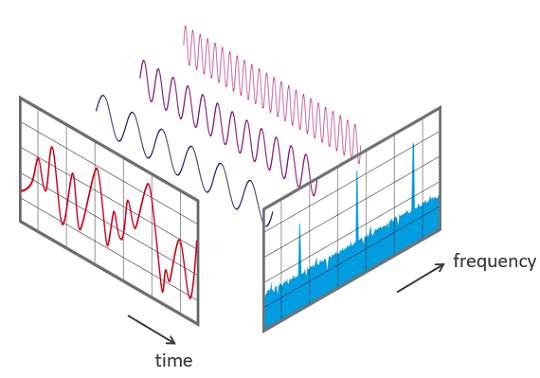
\includegraphics[width=0.5\textwidth]{img/fft_time_freq.png}
    \caption{Time to frequency signal decomposition \source{fftntiaudio}}
    \label{fig:signal-decomposition}
\end{figure}

% REVIEW
Sine and cosine waves are in simple waveforms, they can then be manipulated with relative ease. This process is constantly present in communications due to the transmission of data over wires and radio circuits through signals and most devices nowadays perform it frequently.
\newline

In this introductory chapter, we present a preface on the Fourier Transform in \autoref{sec:continuous-fourier-transform} and describe the discrete version of the Fourier Transform in \autoref{sec:discrete-fourier-transform}, which is the focus of this dissertation. Furthermore, we present the state of the art of the most popular algorithms in \autoref{sec:fast-fourier-transform} and progressively demonstrate how to improve them in the following sections \autoref{sec:stockham-algorithm} and \autoref{sec:radix4-instead-of-radix2}. 
Regarding optimization of the FFT, we then proceed to detail how a complex-to-complex FFT computation can simultaneously transform two distinct real input sequences in \autoref{sec:two-real-inputs-within-one-complex}. At the end of this chapter, in \autoref{sec:2d-fourier-transform} we finalize with an explanation of how one-dimensional algorithms can be applied in the context of 2D input sequences such as an image
% IN CORRECTION STATE % Still regarding optimizations, we proceed on how to a complex-to-complex FFT computation to simultaneously compute two distinct real input sequences. Finally, we describe how the one-dimensional algorithms can be applied in the context of a 2D input sequence such as an image (\autoref{sec:2d-fourier-transform}).

%%%%%%%%%%%%%%%%%%%%%%%%%%%%%%%%%%%%%%%%%%%%%

\section{Continuous Fourier Transform} \label{sec:continuous-fourier-transform}

The Fourier Transform is a mathematical method to decompose a function into frequency components. Intuitively, the Inverse Fourier Transform is the corresponding method to reverse that process and reconstruct the original function from the one in \textit{frequency} domain representation.
% IN CORRECTION STATE: The Fourier Transform is a mathematical method to transform the domain referred to as \textit{time} of a function, to the \textit{frequency} domain, intuitively the Inverse Fourier Transform is the corresponding method to reverse that process and reconstruct the original function from the one in \textit{frequency} domain representation.

Although there are many forms, the Fourier Transform key definition (\cite{adams2020signals}) can be described as \autoref{eq:fourier-transform}.

% Forward Fourier Transform
\begin{equation} \label{eq:fourier-transform}
    \begin{split}
        % Fourier Transform
        X(f) = \int_{-\infty}^{+\infty} x(t)e^{-i f t} dt \\
        % Inverse Fourier Transform
        x(t) = \frac{1}{2\pi} \int_{-\infty}^{+\infty} X(f)e^{-i f t} df \\
    \end{split} %\eqname{Fourier Transform}
\end{equation}

where 

\begin{itemize}
    \item \( X(f), \forall f \in \mathbb{R} \rightarrow \) function in \textit{frequency} domain representation, also called the Fourier Transform of \( x(t) \);
    \item \( x(t), \forall t \in \mathbb{R} \rightarrow \) function in \textit{time} or \textit{space} domain representation;
    \item \( i \rightarrow \) imaginary unit \( i = \sqrt{-1} \).
\end{itemize}

% The definition of \autoref{eq:fourier-transform} integral is only valid if the integral exists for every value of parameter \(f\). 
This formulation shows the usage of a complex-valued domain, making the Fourier Transform range from real to complex values, one complex coefficient per frequency \( X : \mathbb{R} \rightarrow \mathbb{C} \) 
% IN CORRECTION STATE % This formulation shows the usage of complex-valued domain since the imaginary unit \( i \) doesn't represent a value in the set of real numbers, making the fourier transform range from real to complex values, one complex coefficient per frequency \( X : \mathbb{R} \rightarrow \mathbb{C} \) 

If we take into account Euler's formula (\autoref{eq:euler}), we can rewrite the Fourier Transform as represented in \autoref{eq:ft-with-euler}.
% IN CORRECTION STATE % If we take into account Euler's formula \autoref{eq:euler}, we can replace the Fourier Transform for an equivalent, fragmenting the Euler constant for a sine and cosine pair.

% Euler's Formula
\begin{equation} \label{eq:euler}
    e^{ix} = \cos x + i \sin x \\ %\eqname{Euler's Formula} \\
\end{equation}

% Forward Fourier Transform with Euler's Formula
\begin{equation} \label{eq:ft-with-euler}
    X(f) = \int_{-\infty}^{+\infty} x(t) (\cos (-f t) + i \sin (-f t)) dt \\
\end{equation}

Hence, we can break the Fourier Transform apart into two formulas that give each coefficient of the sine and cosine components as functions without dealing with complex numbers.

% Forward Fourier Transform sine and consine
\begin{equation}
    \begin{split}
        X(f) = X_{a}(f) + i X_{b}(f) \\
        X_{a}(f) = \int_{-\infty}^{+\infty} x(t) \cos (f t) dt \\
        X_{b}(f) = \int_{-\infty}^{+\infty} x(t) \sin (f t) dt \\
    \end{split}
\end{equation}


% FIXME: This might also be applied to the Inverse, study this later and try to deduce the correspondant pair of formulas
% NOTE: This is important for future reference

% Fourier's original formulation of the transform did not use complex numbers, but rather sines and cosines. % Chatfield, Chris (2004), The Analysis of Time Series: An Introduction, Texts in Statistical Science (6th ed.), London: Chapman & Hall/CRC, ISBN 9780203491683.

% TODO: explain the formula better
This model of the Fourier Transform applied to infinite domain functions is called Continuous Fourier Transform. % and it is targeted to the calculation of the this transform directly to functions with only finite discontinuities in \( x(t) \).


\section{Discrete Fourier Transform} \label{sec:discrete-fourier-transform}


The Fourier Transform of a finite sequence of equally-spaced samples of a function is called the Discrete Fourier Transform (DFT). It converts a finite set of values in \textit{time}/\textit{space} domain to \textit{frequency} domain representation. It is an usefull version of the Fourier Transform since it deals with a discrete amount of data. This transform is described in \autoref{eq:discrete-fourier-transform}.
% IN CORRECTION STATE % It is an important version of the Fourier Transform since it deals with a discrete amount of data and has the popular algorithm in which is the center of attention of fourier transforms, which can be implemented in machines and be computed by specialized hardware.

% It must show the name AND the number
\begin{equation} \label{eq:discrete-fourier-transform}
    \begin{split}
        % Forward Discrete Fourier Transform
        X_{k} = \sum_{n=0}^{N-1}x_{n} \cdot e^{- \frac{i 2 \pi}{N}kn} \\ %\eqname{Forward Discrete Fourier Transform} \\
        % Inverse Discrete Fourier Transform
        x_{n} = \frac{1}{N} \sum_{k=0}^{N-1}X_{k} \cdot e^{\frac{i 2 \pi}{N}kn} \\ %\eqname{Inverse Discrete Fourier Transform} \\
    \end{split}
\end{equation}

% REVIEW (english)
Notably, the discrete version of the Fourier Transform has some obvious differences since it deals with a discrete time sequence. The first difference is that the sum covers all elements of the input values instead of integrating the infinite domain of the function, but we can also notice that the exponential, similar to the aforesaid, divides the values by \(N\) (\(N\) being the total number of elements in the sequence) due to the inability to look at frequency and time \(ft\) continuously we instead take the \(k\)'th frequency over \(n\).

We can expand this formula as:
% IN CORRECTION STATE % We can have a more simplified expansion of this formula with:

\begin{equation*}
    X_{k} = x_{0} + x_{1}e^{\frac{i 2 \pi}{N}k} + ... + x_{N-1}e^{\frac{i 2 \pi}{N}k(N-1)} \\
\end{equation*}

% FIXME: Maybe the word i want isn't simplified because the equation is getting longer
Having this sum simplified we then only need to resolve the complex exponential, and we can do that by replacing the \(e^{\frac{i 2 \pi}{N}kn}\) by the Euler formula as mentioned before to reduce the maths to a simpler sum of real and imaginary numbers.

% REVIEW (math)
\begin{equation} \label{dft_reduction}
    X_{k} = x_{0} + x_{1} (\cos{b_{1}} + i\sin{b_{1}}) + ... + x_{N-1} (\cos{b_{N-1}} + i\sin{b_{N-1}}) \\
\end{equation}

\begin{equation*}
    \text{where } \\ b_{n} = \frac{ 2 \pi}{N}kn \\
\end{equation*}


Finally, the result will be a complex number.

% \begin{equation*}
%     X_{k} = A_{k} + i B_{k}
% \end{equation*}

% 1. Explicar como funciona a aplicação da DFT a uma sequência (fazer um exemplo para sinais visto que vamos ter que mencionar a frequencia de nyquist)

\paragraph{Example} Let us now follow an example of calculation of the DFT for a sequence \(x\) with N number of elements.

%\pagestyle{empty}
% Plot the cosine wave graph with the sample values
% \begin{figure*}
%     \begin{tikzpicture}
%         \begin{axis}[width=9cm,height=4cm,
%             axis lines = center,
%             axis on top,
%             axis line style={thick},
%             ticklabel style={fill=white,font=\scriptsize, inner sep=1pt},
%             xmin=0, xmax=360,
%             ymin=-1.9, ymax=1.9,
%             % ytick={-2,-1,...,2},
%             % xtick={-2,-1,...,2},
%             legend style={draw=none,fill=white, fill opacity=0.75, 
%                           font=\scriptsize, text opacity=1, inner sep=1pt,
%                           anchor=north east, at={(1,1)}, legend columns=-1},
%             domain=0:360,
%             samples=181,
%             no marks
%                     ]
%         \addplot +[s_orange,thick] {cos(x)};
%         \legend{$\cos(x)$}
%         \end{axis}
%     \end{tikzpicture}
% \end{figure*}

\begin{equation*}
    x = 
    \begin{bmatrix}
        1 & 0.707 & 0 & -0.707 & -1 & -0.707 & 0 & 0.707\\
    \end{bmatrix}
\end{equation*}
\begin{equation*}
    N = 8
\end{equation*}

% REVIEW: Not sure about this phrase
With this sequence, we now want to transform it into the frequency domain, therefore we apply the Discrete Fourier Transform to each element \( x_{n} \rightarrow X_{k} \), thus, for each \(k\)'th element of \(X\) we apply the DFT for every element of \(x\).

% REVIEW: Not sure if i should put intermediate steps in this apply of the DFT
\begin{equation*}
    X_{0} = 1 \cdot e^{- \frac{i 2 \pi}{8} \cdot 0 \cdot 0} \\
        + 0.707 \cdot e^{- \frac{i 2 \pi}{8} \cdot 0 \cdot 1}  \\
        + ...  \\
        + 0.707 \cdot e^{- \frac{i 2 \pi}{8} \cdot 0 \cdot 7} \\
\end{equation*}
\begin{equation*}
    = (0 + 0i)
\end{equation*}
\begin{equation*}
    X_{1} = 1 \cdot e^{- \frac{i 2 \pi}{8} \cdot 1 \cdot 0} \\
        + 0.707 \cdot e^{- \frac{i 2 \pi}{8} \cdot 1 \cdot 1}  \\
        + ...  \\
        + 0.707 \cdot e^{- \frac{i 2 \pi}{8} \cdot 1 \cdot 7} \\
\end{equation*}
\begin{equation*}
    = (4 + 0i)
\end{equation*}

\begin{equation*}
    . . .
\end{equation*}

\begin{equation*}
    X_{7} = 1 \cdot e^{- \frac{i 2 \pi}{8} \cdot 7 \cdot 0} \\
        + 0.707 \cdot e^{- \frac{i 2 \pi}{8} \cdot 7 \cdot 1}  \\
        + ...  \\
        + 0.707 \cdot e^{- \frac{i 2 \pi}{8} \cdot 7 \cdot 7} \\
\end{equation*}
\begin{equation*}
    = (4 + 0i)
\end{equation*}

% TODO: Should i do this ^ for the idft too?

And that will produce our complex-valued output in the frequency domain.
\begin{equation*}
    X = 
    \begin{bmatrix}
        0i & 4+0i & 0i & 0i & 0i & 0i & 0i & 4+0i\\
    \end{bmatrix}
\end{equation*}


% TODO:
% [-] 1. Justify why the hz 1 isn't with just 1 since the input sequence comes from a sampled cosine wave and mention the nyquist limit (Not sure if i want to add this)
%   [-] 1.1. Talk about the properties of the magnitude and phase 
% [x] 2. Perform this calculation as a matrix dot product and that makes it better for the computer to compute
%   [1/2] 2.1 Continue previous example but now with matrix multiplication form
% [ ] 3. Algorithmic preview of the dft
% [x] 4. Last phrase that introduces the next chapter FFT

% NOTE: 2.
\subsection{Matrix multiplication} \label{subsec:matrix-multiplication}
The example shown above is done sequentially as if each frequency component is computed individually, but there is a way to express the DFT using matrix multiplication (\cite{rao2018transform}). Since the operations are done equally without any extra step we can group all analyzing function sinusoids (\(e^{- \frac{i 2 \pi}{N} k n}\)), also referred to as twiddle factors.

% \ref{example1}

\begin{equation*}
    W = 
    \begin{bmatrix}
        \omega_{N}^{0 \cdot 0}     & \omega_{N}^{1 \cdot 0}     & \dots  & \omega_{N}^{(N-1) \cdot 0}     \\
        \omega_{N}^{0 \cdot 1}     & \omega_{N}^{1 \cdot 1}     & \dots  & \omega_{N}^{(N-1) \cdot 1}     \\
        \vdots                     & \vdots                     & \ddots & \vdots                          \\
        \omega_{N}^{0 \cdot (N-1)} & \omega_{N}^{1 \cdot (N-1)} & \dots  & \omega_{N}^{(N-1) \cdot (N-1)} \\
    \end{bmatrix} =
    \begin{bmatrix}
        1      & 1              & \dots  & 1                          \\
        1      & \omega         & \dots  & \omega^{(N-1)}             \\
        \vdots & \vdots         & \ddots & \vdots                     \\
        1      & \omega^{(N-1)} & \dots  & \omega^{(N-1) \cdot (N-1)} \\
    \end{bmatrix}
\end{equation*}
\begin{equation*}
    \text{where } \omega_{N} = e^{- \frac{i 2 \pi}{N}}
\end{equation*}

% FIXME: I dont like the way this two phrases are right now, change later
The substitution variable \(\omega\) allows us to avoid writing extensive exponents. 

The symbol \(W\) represents the transformation matrix of the Discrete Fourier Transform (\cite{rao2018transform}), also called the DFT matrix, and its inverse can be defined as.

\begin{equation*}
    W^{-1} = \frac{1}{N} \cdot
    \begin{bmatrix}
        1      & 1                  & \dots  & 1                              \\
        1      & \omega_{N}         & \dots  & \omega_{N}^{(N-1)}             \\
        \vdots & \vdots             & \ddots & \vdots                         \\
        1      & \omega_{N}^{(N-1)} & \dots  & \omega_{N}^{(N-1) \cdot (N-1)} \\
    \end{bmatrix}
\end{equation*}

\begin{equation*}
    \text{where } \omega_{N} = e^{\frac{i 2 \pi}{N}} \\
\end{equation*}

% By using this matrix multiplication form we can have a more efficient way to compute the DFT.  
We separate the twiddle factors in a matrix and express the DFT as a matrix multiplication between the twiddle factors and the input sequence. When the size is known before the transformation, it is possible to pre-calculate and reuse the matrix of the factors

\begin{equation*}
    X = W \cdot x \\ %\eqname{Matrix DFT} \\
\end{equation*}
\begin{equation*}
    x = W^{-1} \cdot X \\ %\eqname{Matrix IDFT} \\
\end{equation*}

It is also worth noting that normalizing the DFT and IDFT matrix be by  \( \sqrt{N} \) instead of just normalizing the IDFT by \(N\), will make \(W\) a unitary matrix \cite{horn2012matrix}. However, this normalization by \( \sqrt{N} \) is not common in FFT implementations since it is more simple and efficient to normalize the inverse by $N$, than the forward and the inverse by $\sqrt{N}$.

%The advantage of using a unitary matrix is that we only need to reasign the constant substution variable \(\omega_{N}\) to be able to invert the dft, the matrix multiplication stays the same for both DFT and IDFT. 
% FIXME: This phrase isn't good in this context, is contradicting the aforesaid.
%Nevertheless later we will verify that the use of sqrt function isn't desirable for the implementation of any dft.

% NOTE: 2.1.
\paragraph{Example} Continuing the previous example, we can adapt the application of the DFT to the matrix multiplication form.

\begin{equation*}
    W =
    \begin{bmatrix}
        1      & 1              & \dots  & 1               \\
        1      & \omega_{8}     & \dots  & \omega_{8}^{7}  \\
        \vdots & \vdots         & \ddots & \vdots          \\
        1      & \omega_{8}^{7} & \dots  & \omega_{8}^{49} \\
    \end{bmatrix}
\end{equation*}
\begin{equation*}
    \text{where } \omega_{8} = e^{\frac{i 2 \pi}{8}}
\end{equation*}

\begin{equation*}
    X = W \cdot x = W \cdot 
    \begin{bmatrix}
        1      \\
        0.707  \\
        \vdots \\
        0.707  \\
    \end{bmatrix} =
    \begin{bmatrix}
        0      \\
        4+0i  \\
        \vdots \\
        4+0i  \\
    \end{bmatrix}
\end{equation*}


% NOTE: 3. Algorithmic preview of the dft
\hfill \break
% NOTE: 4. Last phrase that introduces the next chapter FFT
% REVIEW: (english) Usage of word conspicuous
It is conspicuous that the complexity time for each complex multiplication of every singular term of the sequence with the complex exponential value is \(O(N^{2})\), hence, the computation of the Discrete Fourier Transform rises exponentially with the sequence length. Therefore, over time new algorithms and techniques were developed to increase the performance of this transform due to its usefulness. 


\section{Fast Fourier Transform} \label{sec:fast-fourier-transform}

The \acrfull{fft} is a family of algorithms that compute the \acrfull{dft} of a sequence, and its inverse, efficiently, since the direct usage of the DFT formulation is too slow for its applications. Thus, FFT algorithms exploit the DFT matrix structure by employing a divide-and-conquer approach (\cite{chu1999inside}) to segment its application.

Over time several variations of the algorithms were developed to improve the performance of the DFT and many aspects were rethought in the way we compute the transform.

\paragraph{}
There are many algorithms and approaches on the FFT family such as the well known Cooley-Tukey \cite{cooley1965algorithm}, known for its simplicity and effectiveness to compute any sequence with size as a power of two, but also Rader's algorithm \cite{rader1968discrete} and Bluestein's algorithm \cite{bluestein1970linear} to deal with prime sized sequences, and even the Split-radix FFT \cite{yavne1968economical} that recursively expresses a DFT of size \(N\) in one DFT of size \(N/2\) and two DFTs of size \(N/4\).
\newline

%%%%%%%%%%%%%%%%%%%%%%%%%%%%%%%%%%%%%%%%%%%%%%%%%%%%%%%%%%%

% TODO: The original DFT complexity
Computing the DFT directly requires $N^{2}$ complex multiplies and $N (N-1)$ complex additions, by using an FFT algorithm to compute the DFT, it only requires $(N/2)\log{(N)}$ complex multiplies and complex additions.

% TODO: 4-pt DFT structure
When we consider a DFT of a sequence of length 4, we can notice that some of the operations involved repeat themselves for the computation of the whole sequence.

In \autoref{eq:dit-op-reuse} we list the required operations to compute the DFT of a sequence with $4$ elements. 

\begin{equation} \label{eq:dit-op-reuse}
    \begin{split}
    X_{0} &= x_{0} + x_{1} + x_{2} + x_{3} \\
    X_{1} &= x_{0} - i \cdot x_{1} - x_{2} + i \cdot x_{3} \\
    X_{2} &= x_{0} - x_{1} + x_{2} - x_{3} \\
    X_{3} &= x_{0} + i \cdot x_{1} - x_{2} - i \cdot x_{3} \\
    \end{split}
\end{equation}

When the operations are grouped together, we have a clear perception of the repetition of the operations, as presented in \autoref{eq:dit-op-reuse-grouped}.

\begin{equation} \label{eq:dit-op-reuse-grouped}
    \begin{split}
    X_{0} &= (x_{0} + x_{2}) + (x_{1} + x_{3}) \\
    X_{1} &= (x_{0} - x_{2}) - i \cdot (x_{1} - x_{3}) \\
    X_{2} &= (x_{0} + x_{2}) - (x_{1} + x_{3}) \\
    X_{3} &= (x_{0} - x_{2}) + i \cdot (x_{1} - x_{3}) \\
    \end{split}
\end{equation}

The FFT takes advantage of the periodic roots of unity values and the repetitive operations to generalize the grouping in \autoref{eq:dit-op-reuse-grouped} for a sequence of size N. This algorithm itself is a multiplication of the input sequence by a sparse matrix (\cite{heckbert1995fourier}). It achieves this by computing the butterfly operations at each stage and storing them to allow the reuse of the intermediate values in the next stage until the DFT is computed for every element.
 \newline


It is worth noting that for power of $2$ sizes, the roots of unity are symmetrical and periodic over $N$, therefore, any twiddle factor $\omega^{k}_{N}$ is equal to $\omega^{k+N}_{N}$ and $-\omega^{k+N/2}_{N}$. For example, in figure \autoref{fig:roots-of-unity-properties} we have the roots of unity for $N = 8$, where $\omega^{0}_{8} = -\omega^{4}_{8}$ and $\omega^{0}_{8} = \omega^{8}_{8}$.
% and where w^{8} will loop over the same w^{0} complex value.
% Example: $\omega^{0}_{8} = -\omega^{4}_{8}$ and $\omega^{0}_{8} = \omega^{8}_{8}$  

\begin{figure}[h] 
    \centering
    \includegraphics[width=0.45\textwidth]{img/roots_of_unity_properties.png}
    \caption{Roots of unity with $N = 8$ \source{heckbert1995fourier}}
    \label{fig:roots-of-unity-properties}
\end{figure}

%%%%%%%%%%%%%%%%%%%%%%%%%%%%%%%%%%%%%%%%%%%%%%%%%%%%%%%%%%%

\autoref{subsec:radix-2-decimation-in-time-fft} and \autoref{subsec:radix-2-decimation-in-frequency-fft} focus on the Cooley–Tukey algorithm for sequences with power of $2$ sizes. In \autoref{subsec:radix-2-decimation-in-time-fft} we describe how to generalize the FFT algorithm with decimation in time, and explain where this algorithm reduces the computational cost of the DFT. Moreover, in \autoref{subsec:radix-2-decimation-in-frequency-fft} we present another well-known variation of this algorithm with decimation in frequency.

%The next two sections focus on the Cooley–Tukey algorithm, most specifically the radix-2 decimation-in-time (DIT) FFT and radix-2 decimation-in-frequency (DIF) FFT, both requiring the input sequence to have a power of two size. These two variations of the Cooley–Tukey algorithm represent the most popular implementations of what an individual in need to implement FFT will most likely be familiar with.

\subsection{Radix-2 Decimation-in-Time FFT} \label{subsec:radix-2-decimation-in-time-fft}

% 1. Explain the objective and what the DIT term means in the applied algorithm
% (is one of the most used)

The Radix-2 Decimation-in-Time FFT algorithm rearranges the computation of a DFT of size N into two DFTs of size N/2, one as a sum over the even indexed elements and the other as a sum over the odd indexed elements. Cooley and Tukey proved this possibility of dividing the DFT computation into two smaller DFTs by exploiting this division (\cite{cooley1965algorithm}), as presented in \autoref{eq:dit}. Hence, it is hinted the recursive definition of this formulation on both DFT of size $N/2$.

\begin{equation} \label{eq:dit}
    \begin{split}
        X_{k} &= \sum_{n=0}^{N-1}x_{n} \cdot \omega_{N}^{kn} \\
        X_{k} &= \sum_{n=0}^{N/2-1}x_{2n} \cdot \omega_{N}^{k(2n)} + \sum_{n=0}^{N/2-1}x_{2n+1} \cdot \omega_{N}^{k(2n+1)} \\
        X_{k} &= \sum_{n=0}^{\frac{N}{2}-1}x_{2n} \cdot \omega_{N/2}^{kn} + \omega_{N}^{k} \sum_{n=0}^{\frac{N}{2}-1}x_{2n+1} \cdot \omega_{N/2}^{kn} \\
    \end{split}
\end{equation}

%%%%%%%%%%%%%%%%%%%%%%%%%%%%%%%%%%%%%

\begin{equation*}
    \text{where } \omega_{N} = e^{\frac{i 2 \pi}{N}}
\end{equation*}


%%%%%%%%%%%%%%%%%%%%%%%%%%%%%%%%%%%%%%%%%%%%%%%%%%%%%

This formulation segments the full-sized DFT into two $N/2$ sized DFTs of the even and odd indexed elements where the latter is multiplied by a factor called twiddle $\omega_{N}^{k}$. We can notice that in the $N/2$ sub-transform, the twiddle factors of $\omega^{k}_{N/2}$ will be periodic for $k=0,1,...,N-1$. This periodicity can also be noticed in \autoref{eq:dit-op-reuse-grouped} within the sub-transforms of the even and odd elements.

%Nevertheless, this segmentation alone does not change the number of operations of the DFT.


This algorithm is a Radix-2 Decimation-in-Time in the sense that elements are regrouped into 2 sub-transforms, and the decomposition reduces the time values to the frequency domain. The understanding of this algorithm comes from the recursive application of \autoref{eq:dit}, to compute the FFT for all the values of the input sequence. \autoref{fig:dit-fft} illustrates the composition of the sub-transforms, where the DFTs of size $N/2$ can be replaced with the same decomposition of even and odd sub-transforms.


\begin{figure}[h] 
    \centering
    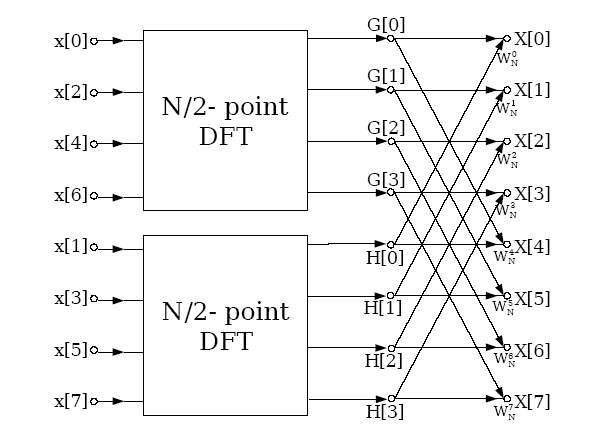
\includegraphics[width=0.5\textwidth]{img/dit_fft.png}
    \caption{Radix-2 Decimation-in-Time FFT \source{jones2014digital}}
    \label{fig:dit-fft}
\end{figure}


Effectively, the main building block in the FFT is the butterfly operation of $2$ elements since it calculates intermediate values at each stage to compute the FFT of the whole sequence. This butterfly operation resembles the computation of a length-2 DFT but with a shifted element according to the sub-transform size

This butterfly, without any reuse of the twiddle factor, corresponds to:

\begin{equation} \label{eq:dit}
    \begin{split}
    A = a + b \cdot \omega_{N}^{k} \\
    B = a + b \cdot \omega_{N}^{k+N/2} \\
    \end{split}
\end{equation}

\begin{equation*}
    \text{where } A = x_{k} \\ \text{and } B = x_{k+N/2} \\
\end{equation*}


Yet, since the roots of unity for $k$ and $k+N/2$ over $N$ are symmetrical, as illustrated in \autoref{fig:roots-of-unity-properties}, we may re-express this butterfly in terms of the same twiddle factor $\omega_{N}^{k}$, such that $\omega_{N}^{k+N/2}$ will be equal to $-\omega_{N}^{k}$ (\cite{jones2014digital}). With this said, this Cooley-Tukey butterfly (\cite{chu1999inside}) reuses the same twiddle factor, as illustrated in \autoref{fig:dit-butterfly}.


\begin{figure}[H] 
    \centering
    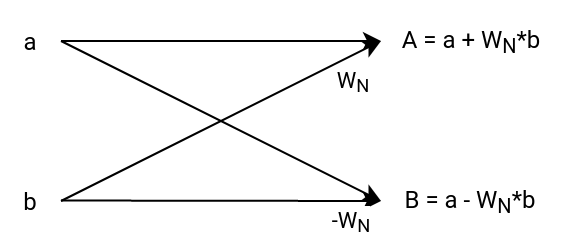
\includegraphics[width=0.5\textwidth]{img/dit_butterfly.png}
    \caption{Cooley-Tukey butterfly}
    \label{fig:dit-butterfly}
\end{figure}

% "Whereas direct computation of all N DFT frequencies according to the DFT equation would require N2 complex multiplies and N2−N complex additions (for complex-valued data), by reusing the results of the two short-length DFTs as illustrated in Figure, the computational cost is now" 

The complexity work of the algorithm is distributed within the DIT approach which decomposes each DFT by 2 having \(\log{(N)}\) stages \cite{smith2007mathematics}. There are $N$ complex multiplications needed for each stage of the DIT decomposition, therefore, the multiplication complexity for a $N$ sized DFT is reduced from $O(N^{2})$ to $O(N \log{(N)})$.
\newline

%%%%%%%%%%%%%%% BIT REVERSAL PERMUTATION %%%%%%%%%%%%%%%

% Why do we need the bit reverse
The splitting of the DFT into two smaller half-sized DFTs causes the original input sequence to require a special reordering to pass the even and odd numbers into, and when this algorithm is applied recursively, this reordering is always needed, so in the end, we need a special order for the input elements, fortunately, as noted by \cite{thong1981algebraic} this order corresponds to the bit reversed indices of the sequence, therefore, we need to apply a bit reverse permutation to the elements of the input sequence.
%One consequence of using this algorithm is that the input sequence is required to be in natural order to be able to, therefore, we need to apply some kind of data reordering to the input sequence.
%therefore, applying the inverse on the Fourier Transform of a sequence won't return the same elements.

% What is the bit reverse
The bit reversal of the input sequence corresponds to the permutation of swapping the position of the elements to its bit reversed index, as illustrated in \autoref{fig:bit-reverse-permutation}. The $bit\_reverse$ of an index depends directly on the indexing domain of the input sequence, therefore, it needs the size $N$, or more precisely the $\log{(N)}$ value, to use as a reference to reverse the bit order while maintaining the value within the sequence range.

\begin{figure}[h] 
    \centering
    \includegraphics[width=0.5\textwidth]{img/bit_reverse_permutation.png}
    \caption{Bit reverse permutation}
    \label{fig:bit-reverse-permutation}
\end{figure}

For example, for a sequence of size 16, we have some index with $\log{16}$ bits $b_1 b_2 b_3 b_4$, which corresponds to the bit reversed index as $b_4 b_3 b_2 b_1$.

For the DIT algorithm, we apply the bit reversal permutation to the input sequence to return a natural order result.
% For the DIT algorithm we apply the bit reverse permutation to the input sequence to return a natural order result.
% IN CORRECTION STATE % Both the DIT and DIF FFT algorithms require this bit reversal permutation step, but in the case of the DIT we bit reverse the input sequence and on the DIF we apply it to the output, to result in a natural order sequence.

There are many implementations of the bit reversal, and since it is quite simple, any decent version can be used in regard to this FFT algorithm since it is not the main bottleneck. An algorithm such as \autoref{alg:bit-reverse} can be used for the $bit\_reverse$ function or any other efficient alternatives (\cite{prado2004new}).
\newline 

\SetKwComment{Comment}{/* }{ */}
\RestyleAlgo{ruled}
\begin{algorithm}[H]
    \caption{Bit reverse} \label{alg:bit-reverse}
    \KwData{Integer $i$}
    \KwResult{Bit reversed integer $i$}

    $n \gets 0$ 
    
    \ForEach{$i = 0$ \textbf{to} $\log{(N)}-1$}{
        $n \gets n << 1$\;
        $n \gets n | (i \& 1)$\;
        $i \gets i >> 1$\;
    }
    \textbf{return} $i$\;
\end{algorithm}
% \newline

In practice, \autoref{alg:dit} demonstrates the aforesaid with an iterative DIT implementation for the forward FFT. To compute its inverse the algorithm is the same, we just need to use the twiddle factor with a positive exponent $w_{m} \gets \exp(2\pi i / m)$.

Although this algorithm is congruent with a code implementation, it is worth noting that the input sequence can either have real or complex numbers, since the arithmetic is the same for both domains the only thing that needs to be specialized is the operator overloading in the innermost loop. 
\newline

% 3. Algorithmic overview
\SetKwComment{Comment}{/* }{ */}
\RestyleAlgo{ruled}
\begin{algorithm}[H]
    \caption{Radix-2 Decimation-in-Time Forward FFT} \label{alg:dit}
    \KwData{Sequence $in$ with size $N$ power of 2 }
    \KwResult{Sequence $out$ with size $N$ with the DFT of the input}

    \Comment{Bit reversal step}
    \ForEach{$i = 0$ \textbf{to} $N-1$}{
        $out[$bit\_reverse$(i)] \gets in[i]$
    }

    \Comment{FFT}
    \ForEach{$s = 1$ \textbf{to} $\log{(N)} $}{
        $m \gets 2^{s}$\;
        $w_{m} \gets \exp(-2\pi i / m)$\;
        \ForEach{$k = 0$ \textbf{to} $N-1$ \textbf{by} $m$}{
            $w \gets 1$\;
            \ForEach{$j = 0$ \textbf{to} $m/2$}{
                $bw \gets w \cdot out[k + j + m/2] $\;
                $a \gets out[k + j] $\;
                $out[k + j] \gets a + bw$\;
                $out[k + j + m/2] \gets a - bw$\;
                $w \gets w \cdot w_{m}$\;
            }
        }
    }
    \textbf{return} $out$\;
\end{algorithm}


\subsection{Radix-2 Decimation-in-Frequency FFT}  \label{subsec:radix-2-decimation-in-frequency-fft}

% 1. Explain the objective and what the DIF term means in the applied algorithm
The Radix-2 Decimation-in-Frequency FFT algorithm is very similar to the DIT approach, it is based on the same principle of divide-and-conquer, however, it rearranges the original \acrshort{dft} into the computation of two transforms, one with the even indexed elements and other with the odd indexed elements, as demonstrated in \autoref{eq:dif}.

\begin{equation}
    \begin{split}
        X_{k} &= \sum_{n=0}^{N-1}x_{n} \cdot \omega_{N}^{kn} \\
        X_{k} &= \sum_{n=0}^{N/2-1}x_{n} \cdot \omega_{N}^{kn} + \sum_{n=0}^{N/2-1}x_{n+N/2} \cdot \omega_{N}^{k(n+N/2)} \\
        X_{k} &= \sum_{n=0}^{N/2-1}x_{n} \cdot \omega_{N}^{kn} + (-1)^k \times \sum_{n=0}^{N/2-1}x_{n+N/2} \cdot \omega_{N}^{kn} \\
        X_{k} &= \sum_{n=0}^{N/2-1} (x_{n} + (-1)^{k} \times x_{n + \frac{N}{2}}) \cdot \omega_{N/2}^{kn} \\
    \end{split}
\end{equation}

% w^kn + w^kN/2
% w^kN/2 = (-1)^k
% (-1)^k
% $-1$ raised to an even number is always $1$ and raised to an odd number is $-1$.

\begin{equation} \label{eq:dif}
    \begin{split}
        X_{2k} &= \sum_{n=0}^{N/2-1} (x_{n} + x_{n + \frac{N}{2}}) \cdot \omega_{N}^{2kn} = \sum_{n=0}^{N/2-1} (x_{n} + x_{n + \frac{N}{2}}) \cdot \omega_{N/2}^{kn} \\
        X_{2k+1} &= \sum_{n=0}^{N/2-1} (x_{n} + x_{n + \frac{N}{2}}) \cdot \omega_{N}^{(2k+1)n} = \sum_{n=0}^{N/2-1} ((x_{n} - x_{n + \frac{N}{2}}) \cdot \omega_{N/2}^{kn}) \cdot \omega_{N}^{n} \\
    \end{split}
\end{equation}

\begin{equation*}
    \text{where } \omega_{N} = e^{\frac{i 2 \pi}{N}}
\end{equation*}


As explained in the previous section, the computational savings for this algorithm come from exploiting the DFT to reuse repeated calculations by storing intermediate terms in between stages.


This algorithm is a Radix-2 Decimation-in-Frequency since the DFT is decimated into two distinct smaller DFT's and the frequency samples will be computed separately in different groups as if the regrouping of the DFTs would reduce directly to the frequency domain. The understanding of this algorithm comes from the recursive application of \autoref{eq:dif}, to compute the FFT for all the values of the input sequence. \autoref{fig:dif-fft} illustrates the composition of the transforms, where the DFTs of size $N/2$ can be replaced with the same decomposition in two transforms for the even and odd elements.

\begin{figure}[h] 
    \centering
    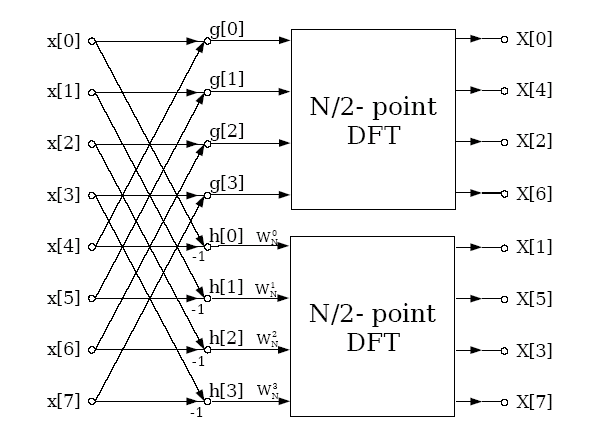
\includegraphics[width=0.5\textwidth]{img/dif_fft.png}
    \caption{Radix-2 Decimation-in-Frequency FFT \source{jones2014digital}}
    \label{fig:dif-fft}
\end{figure}



Similarly to the DIT version, the DFT can be recursively reduced by the DIF algorithm until there is only the computation of a length-2 DFT. At each stage, it is applied the Gentleman-Sande butterfly operation (\cite{chu1999inside}) with a shifted element according to the sub-transform size, as illustrated in \autoref{fig:dif-butterfly}.

% Effectively, the main building block in the FFT is the butterfly operation of $2$ elements, since it calculates intermediate values each stage to compute the FFT of the whole sequence. This butterfly operation resembles the computation of a length-2 DFT but with a shifted element according to the sub-transform size

% NOTE: Handmade since there wan't one that had exacly what i wanted
\begin{figure}[h]
    \centering
    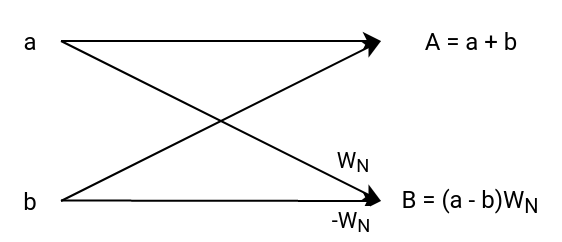
\includegraphics[width=0.5\textwidth]{img/dif_butterfly.png}
    \caption{Gentleman-Sande butterfly}
    \label{fig:dif-butterfly}
\end{figure}

Since this algorithm has similarities with the DIT, its complexity also lives to this similarity, maintaining the same \(O(N \log{(N)})\) for the number of complex multiplications. 
Although they look different, \autoref{fig:dif-butterfly} and \autoref{fig:dit-butterfly} have the same number of operations $1$ addition $1$ subtraction, and $1$ complex multiplication.

% FIXME: The complexity work within the algorithm is distributed with the DIT approach which decomposes each DFT by 2 having \(\log{(N)}\) stages \cite{smith2007mathematics} while there are approximately \(N\) complex multiplications needed for each stage of the DIT decomposition, therefore, the multiplication complexity for a \(N\) sized DFT is reduced from \(O(N^{2})\) to \(O(N \log{(N)})\) without any programming specific optimizations.

Unlike DIT, the DIF algorithm applies bit reversal permutation (\autoref{fig:bit-reverse-permutation}) to the output sequence to produce a natural order result.

In practice, \autoref{alg:dif} demonstrates the aforesaid with an iterative representation of a possible implementation. To compute its inverse the algorithm is the same, we just need to use the twiddle factor with a positive exponent $w_{m} \gets \exp(2\pi i / m)$.
Although this algorithm is congruent with a code implementation, it is worth noting that the input sequence can either have real or complex numbers, since the arithmetic is the same for both domains the only thing that needs to be specialized is the operator overloading in the innermost loop.

% 3. Algorithmic overview
\SetKwComment{Comment}{/* }{ */}
\RestyleAlgo{ruled}
\begin{algorithm}[H]
    \caption{Radix-2 Decimation-in-Frequency Forward FFT} \label{alg:dif}
    \KwData{Sequence $in$ with size $N$ power of 2 }
    \KwResult{Sequence $out$ with size $N$ with the DFT of the input}

    \Comment{FFT}
    \ForEach{$s = 0$ \textbf{to} $\log{(N)}-1 $}{
        $gs \gets N \gg s$\;
        $w_{gs} \gets \exp(2\pi i / gs)$\;
        \ForEach{$k = 0$ \textbf{to} $N-1$ \textbf{by} $gs$}{
            $w \gets 1$\;
            \ForEach{$j = 0$ \textbf{to} $gs/2$}{
                $a \gets in[k + j + gs/2] $\;
                $b \gets in[k + j] $\;
                $in[k + j] \gets a + b$\;
                $in[k + j + gs/2] \gets (a - b) \cdot w$\;
                $w \gets w \cdot w_{gs}$\;
            }
        }
    }
    
    \Comment{Bit reversal step}
    \ForEach{$i = 0$ \textbf{to} $N-1$}{
        $out[$bit\_reverse$(i)] \gets in[i]$
    }

    \textbf{return} $out$\;
\end{algorithm}


Nowadays, there is a lot more to the computation of FFTs than just the basic radix-2 Cooley-Tukey algorithm described previously. As seen by a large amount of current literature, there are more algorithms, variations, and improvements that enhance the computation of this transform in many aspects. Choosing the right conditions enhances the calculation of the performance of this primitive, especially for specific systems (\cite{bengtsson2020development} and \cite{mermer2003efficient}). 

One could optimize the FFT in many ways, and in the next section, we introduce a power of $2$ sizes algorithm called radix-2 Stockham, a natural order algorithm without explicit bit reversal permutation.


\section{Stockham algorithm} \label{sec:stockham-algorithm}


Despite existing already existing fast solutions for index bit reversal (\cite{prado2004new}), this \textit{shuffle} step still weighs the algorithms with extra overhead. The Stockham algorithm is an auto-sort algorithm that eliminates the need to have the bit reversal permutation to output a natural order result. It does this by taking advantage of a reordering of the elements (\cite{govindaraju2008high}) in between stages, as illustrated in \autoref{fig:dif-elements-composition}.

\begin{figure}[h] 
    \centering
    \includegraphics[width=0.5\textwidth]{img/dif_elements_composition.png}
    \caption{Chain of even and odd compositions over each stage for a natural order DIF}
    \label{fig:dif-elements-composition}
\end{figure}
% Caption: Chain of compositions over each stage for a natural order DIF

The natural order elements are composed stage by stage and the butterfly computations stay the same, so this approach takes advantage of the Cooley-Tukey algorithm and turns it into a more suitable form for highly parallelizable hardware such as GPUs, making it a best fit for our implementation in a GPU programmable language. \newline

When the butterflies are performed, the even and odd elements are composed in such a way that the elements will be in natural order. This composition follows the indexing scheme described in \autoref{eq:nat_order_even_indexing}.

\begin{equation} \label{eq:nat_order_even_indexing}
    x[q + 2*p] = y[q + p] \\
\end{equation}
\begin{equation} \label{eq:nat_order_odd_indexing}
    x[q + 2*p + 1] = y[q + p + m] \\
\end{equation}

Where $x$ and $y$ are alternated sequences for read and write over each stage, $q$ corresponds to the sub FFT offset in this stage, $p$ is the index of the sub \acrshort{fft} element shift for the current butterfly being computed, and finally $m$ corresponds to the size of the sub FFT divided by 2.

This algorithm requires the use of two alternating sequences for reading and writing the elements for each stage since there is the possibility of reading from a position that it has already been written. That said, it is ensured that at each stage no values are read to which the result of a butterfly has already been saved.
Finally, as a consequence of using these alternate sequences, the final result will be in the last sequence we wrote in the last stage, hence, we can determine which sequence the result is based on the number of stages $\log{(N)}.
\newline

%, the read of an element which has been altered before read in a given stage. In the end the result will be in the last sequence we wrote to.


This algorithm is described in \autoref{alg:stockham-dif}. To compute its inverse the algorithm is the same, we just need to use the twiddle factor with a positive exponent $w_{p} = \exp(2 * \pi * i * p / gs)$. This version may seem visually different from the Cooley Tukey, however, it preserves the algorithm logic and gets rid of the bit reversal permutation. One main consequence of this algorithm is the requirement of additional space complexity for the alternated read and write access within every stage. %Nevertheless, this does not affect our GPU implementations in the next chapters since they already require this constraint.


% TODO: Devo incluir a versão inversa? é que como so é preciso mudar um sinal nao acho que valha a pena e so fica mais verboso

% FIXME: O if statement tem um end antes do else nao sei como retirar

% 3. Algorithmic overview
\SetKwComment{Comment}{/* }{ */}
\RestyleAlgo{ruled}
\begin{algorithm}[H]
    \caption{Stockham Radix-2 Decimation-in-Frequency Forward FFT} \label{alg:stockham-dif}
    \KwData{Sequence pingpong0 with size $N$ power of 2}
    \KwResult{Sequence $out$ with size $N$ with the DFT of the input}

    \ForEach{$s = 0$ \textbf{to} $\log{(N)}-1 $}{
        $gs \gets N \gg s$\;
        $stride \gets 1 \ll s$\;
        %$w_{gs} \gets \exp(2\pi i / gs)$\;
        \ForEach{$i = 0$ \textbf{to} $N-1$}{
            $p \gets i $ div $ stride $\;
            $q \gets i $ mod $ stride $\;
            $w_{p} = \exp(-2 * \pi * i * p / gs)$\;
            % HERE
            \eIf{$stage $ mod $ 2 == 0$} {
                $a \gets pingpong0[q + s*(p + 0)] $\;
                $b \gets pingpong0[q + s*(p + gs/2)] $\;
                \Comment{Perform butterfly}
                $pingpong1[q + s*(2*p + 0)] = a + b$\;
                $pingpong1[q + s*(2*p + 1)] = (a-b) * w_{p}$\;
            } {
                $a \gets pingpong1[q + s*(p + 0)] $\;
                $b \gets pingpong1[q + s*(p + gs/2)] $\;
                \Comment{Perform butterfly}
                $pingpong0[q + s*(2*p + 0)] = a + b$\;
                $pingpong0[q + s*(2*p + 1)] = (a-b) * w_{p}$\;
            }
        }
    }
    \eIf{$\log{(N)} $ mod $ 2 == 0$}{
        \textbf{return} pingpong1\;
    } {
        \textbf{return} pingpong0\;
    }
\end{algorithm}
\newline

\paragraph{}
This algorithm description will give us a solid code base to use as reference when implementing it on the GPU, mainly due to the way we are indexing and the usage of alternating read write sequences.

%Despite this algorithm description being an algorithmic or more close to a CPU implementation than GPU it will give us a solid structure to use as reference for our comparison subjects since it is feasible to make a similar implementation for GPGPU programmable languages due to the way of indexing and the usage of alternating sequences.

\section{Radix-4 instead of Radix-2} \label{sec:radix4-instead-of-radix2}
% Introduce the topic
% How it works/Explain
% - With radix-4 we segment the transform into 4 distinct transforms
% - Perform a 4 point butterfly (dragonfly) each stage
% Algorithm
% Pros and Cons
% - Less stages, which might be beneficial on the GPU (less synchronization steps)
% - Probably higher kernel sizes on the GPU
% - Main constraint is FFT size
% - Theres a bypas of the FFT size constrain but it turns the implementation more complex the higher the radix
After presenting the radix-2 version of the Stockham algorithm, in this section we expand the application of this algorithm for higher radix such as radix-4 and consequently reflect on its advantages and disadvantages.

We've discussed multiple radix-2 approaches, however, we can explore a wide range of alternatives when we get into higher radices other than just radix-2. These FFT algorithms can use higher radix for better performance and even mixed radix \cite{singleton1969algorithm} for a wider range of input sequence sizes.

Rearranging the Stockham algorithm to radix-4 upgrades the computation of the butterflies while reducing the number of stages which will be crucial in later sections.
The radix-4 performs the work of two radix-2 iterations with less memory accesses (\cite{bailey1988high}).

Theoretically, radix-4 formulation can be twice as fast as a radix-2 \cite{hussain2010evaluation} since it only takes half the stages with more complexity in the butterflies which are sometimes called dragonflies. Additionally, we can use less multiplications with better factorizations (\cite{marti2009radix}).

% How it works/Explain
The radix-4 Stockham splits the FFT of size $N$ into four sub-transforms of size $N/4$ each stage, therefore this algorithm only features $log(N)/2$ stages and requires the size to be power of $4$. Since this is a natural order algorithm the computation of the dragonfly includes the reordering of the elements in natural order at every stage, as illustrated in \autoref{fig:radix4-stockham-stage}.

\begin{figure}[h] 
    \centering
    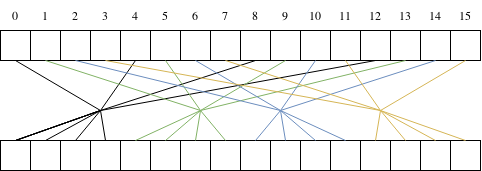
\includegraphics[width=0.6\textwidth]{tese/img/radix4_stockham.png}
    \caption{Illustration of a stage in radix-4 Stockham with each color representing a radix-4 butterfly computation}
    \label{fig:radix4-stockham-stage}
\end{figure}


The dragonfly for this algorithm is illustrated in \autoref{fig:radix4-dragonfly} and its computation involves 4 elements that compute $2$ stages of $2$ radix-2 butterflies.

In \autoref{eq:forward-radix-4-dragonfly} is presented the forward radix-4 dragonfly operations and in \autoref{eq:inverse-radix-4-dragonfly} its inverse.

% TODO: Redo this image with the formulas
% NOTE: 
\begin{figure}[H]
    \centering
    \includegraphics[width=0.6\textwidth]{tese/img/dragonfly.png}
    \caption{Radix-4 FFT butterfly structure \source{marti2009radix}}
    \label{fig:radix4-dragonfly}
\end{figure}

\begin{equation} \label{eq:forward-radix-4-dragonfly}
    \begin{split}
        A &= (a+c) + (b+d) \\
        B &= ((a-c) - i(b-d)) \times \omega_{N}^{p} \\
        C &= ((a+c) -  (b+d)) \times \omega_{N}^{2p} \\
        D &= ((a-c) + i(b-d)) \times \omega_{N}^{3p} \\
    \end{split}
\end{equation}

\begin{equation} \label{eq:inverse-radix-4-dragonfly}
    \begin{split}
        A &= (a+c) + (b+d) \\
        B &= ((a-c) + i(b-d)) \times \omega_{N}^{-p} \\
        C &= ((a+c) -  (b+d)) \times \omega_{N}^{-2p} \\
        D &= ((a-c) - i(b-d)) \times \omega_{N}^{-3p} \\
    \end{split}
\end{equation}

With each stage, the dragonflies are calculated and the elements are reordered similarly to the radix-2 Stockham algorithm. In the end, we get the forward radix-4 Stockham algorithm \autoref{alg:radix4-stockham-forward}. The inverse algorithm is similar, but instead uses the inverse dragonfly as presented in \autoref{eq:inverse-radix-4-dragonfly}.

% Forward
\SetKwComment{Comment}{/* }{ */}
\RestyleAlgo{ruled}
\begin{algorithm}[H]
    \caption{Stockham Radix-4 Decimation-in-Frequency Forward FFT} \label{alg:radix4-stockham-forward}
    \KwData{Sequence pingpong0 with size $N$ power of 4}
    \KwResult{Sequence $out$ with size $N$ with the DFT of the input}

    \ForEach{$stage = 0$ \textbf{to} $\log{(N)}/2-1 $}{
        $n \gets 1 \ll (((\log{(N)}/2) - stage)*2)$\;
        $s \gets 1 \ll (stage*2)$\;
        
        $n0 \gets 0$\;
        $n1 \gets n/4$\;
        $n2 \gets n/2$\;
        $n3 \gets n1 + n2$\;
        
        % FIXME: Acho que acho é N/4-1 e no radix-2 é N72
        \ForEach{$i = 0$ \textbf{to} $N-1$}{
            $p \gets i $ div $ s $\;
            $q \gets i $ mod $ s $\;
            
            $w_{1p} = \exp(-2 * \pi * i * p / n)$\;
            $w_{2p} = w_{1p} * w_{1p}$\;
            $w_{3p} = w_{1p} * w_{2p}$\;
            
            \eIf{$stage $ mod $ 2 == 0$}{
                $a \gets pingpong0[q + s*(p + n0))] $\;
                $b \gets pingpong0[q + s*(p + n1)] $\;
                $c \gets pingpong0[q + s*(p + n2)] $\;
                $d \gets pingpong0[q + s*(p + n3)] $\;
                
                \Comment{Perform dragonfly}
                $pingpong1[q + s*(4*p + 0)] = a + c + b + d$\;
                $pingpong1[q + s*(4*p + 1)] = w_{1p} * ((a-c)-(b-d)*\sqrt{-1})$\;
                $pingpong1[q + s*(4*p + 2)] = w_{2p} * ((a+c)-(b+d))$\;
                $pingpong1[q + s*(4*p + 3)] = w_{3p} * ((a-c)+(b-d)*\sqrt{-1})$\;
            } {
                $a \gets pingpong1[q + s*(p + n0))] $\;
                $b \gets pingpong1[q + s*(p + n1)] $\;
                $c \gets pingpong1[q + s*(p + n2)] $\;
                $d \gets pingpong1[q + s*(p + n3)] $\;
                
                \Comment{Perform dragonfly}
                $pingpong0[q + s*(4*p + 0)] = a + c + b + d$\;
                $pingpong0[q + s*(4*p + 1)] = w_{1p} * ((a-c)-(b-d)*\sqrt{-1})$\;
                $pingpong0[q + s*(4*p + 2)] = w_{2p} * ((a+c)-(b+d))$\;
                $pingpong0[q + s*(4*p + 3)] = w_{3p} * ((a-c)+(b-d)*\sqrt{-1})$\;
            }
            %\EndIf
        }
    }
    \eIf{$\log{(N)} $ mod $ 2 == 0$}{
        \textbf{return} pingpong1\;
    } {
        \textbf{return} pingpong0\;
    }
\end{algorithm}


% Inverse
% \SetKwComment{Comment}{/* }{ */}
% \RestyleAlgo{ruled}
% \begin{algorithm}[H]
%     \caption{Stockham Radix-4 Decimation-in-Time Inverse FFT} \label{alg:radix4-stockham-inverse}
%     \KwData{Sequence pingpong0 with size $N$ power of 4}
%     \KwResult{Sequence $out$ with size $N$ with the DFT of the input}

%     \ForEach{$stage = 0$ \textbf{to} $\log{(N)}/2-1 $}{
%         $n \gets 1 \ll (((\log{(N)}/2) - stage)*2)$\;
%         $s \gets 1 \ll (stage*2)$\;
        
%         $n0 \gets 0$\;
%         $n1 \gets n/4$\;
%         $n2 \gets n/2$\;
%         $n3 \gets n1 + n2$\;
        
%         % FIXME: Acho que acho é N/4-1 e no radix-2 é N72
%         \ForEach{$i = 0$ \textbf{to} $N-1$}{
%             $p \gets i $ div $ s $\;
%             $q \gets i $ mod $ s $\;
            
%             $w_{1p} = \exp(2 \pi *  i * p / n)$\;
%             $w_{2p} = w_{1p} * w_{1p}$\;
%             $w_{3p} = w_{1p} * w_{2p}$\;
            
%             \eIf{$stage $ mod $ 2 == 0$}{
%                 $a \gets pingpong0[q + s*(p + n0))] $\;
%                 $b \gets pingpong0[q + s*(p + n1)] $\;
%                 $c \gets pingpong0[q + s*(p + n2)] $\;
%                 $d \gets pingpong0[q + s*(p + n3)] $\;
                
%                 \Comment{Perform dragonfly}
%                 $pingpong1[q + s*(4*p + 0)] = a + c + b + d$\;
%                 $pingpong1[q + s*(4*p + 1)] = w_{1p} * ((a-c)+(b-d)*\sqrt{-1})$\;
%                 $pingpong1[q + s*(4*p + 2)] = w_{2p} * ((a+c)-(b+d))$\;
%                 $pingpong1[q + s*(4*p + 3)] = w_{3p} * ((a-c)-(b-d)*\sqrt{-1})$\;
%             } {
%                 $a \gets pingpong1[q + s*(p + n0))] $\;
%                 $b \gets pingpong1[q + s*(p + n1)] $\;
%                 $c \gets pingpong1[q + s*(p + n2)] $\;
%                 $d \gets pingpong1[q + s*(p + n3)] $\;
                
%                 \Comment{Perform dragonfly}
%                 $pingpong0[q + s*(4*p + 0)] = a + c + b + d$\;
%                 $pingpong0[q + s*(4*p + 1)] = w_{1p} * ((a-c)+(b-d)*\sqrt{-1})$\;
%                 $pingpong0[q + s*(4*p + 2)] = w_{2p} * ((a+c)-(b+d))$\;
%                 $pingpong0[q + s*(4*p + 3)] = w_{3p} * ((a-c)-(b-d)*\sqrt{-1})$\;
%             }
%             %\EndIf
%         }
%     }
%     \eIf{$\log{(N)} $ mod $ 2 == 0$}{
%         \textbf{return} pingpong1\;
%     } {
%         \textbf{return} pingpong0\;
%     }
% \end{algorithm}

\section{Two real inputs within one complex} \label{sec:two-real-inputs-within-one-complex}
% TWO REAL FFTs WITHIN ONE COMPLEX INPUT
\paragraph{}
It is possible that in the case of an application there is a requirement to compute multiple real FFTs at once. Although we may simply invoke another FFT computation, we can optimize this step by computing multiple FFTs in the context of the same transform.

We can take advantage of the complex input of our implementation to encode multiple real values to avoid extra explicit FFTs. Since the input has elements in a complex format, but the values are real, we only use the real component of the element, therefore, the output of the inverse also contains the complex with only the real component, as illustrated in \autoref{fig:fft-1-real-complex}.

\begin{figure}[H] 
    \centering
    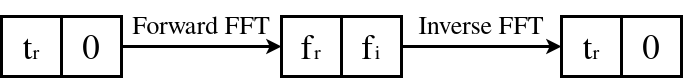
\includegraphics[width=0.6\textwidth]{tese/img/results/fft_1_real_complex.png}
    \caption{FFT for an element without an imaginary part}
    \label{fig:fft-1-real-complex}
\end{figure}

% TODO: Present the pack and Unpack formulas
Based on this, we can reuse the imaginary part of the complex with a meaningful value other than $0$, as illustrated in \autoref{fig:fft-2-real-complex}.

\begin{figure}[H] 
    \centering
    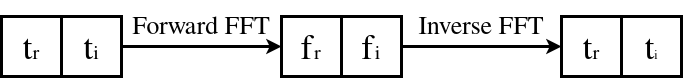
\includegraphics[width=0.6\textwidth]{tese/img/results/fft_2_real_complex.png}
    \caption{FFT for an element with an imaginary part}
    \label{fig:fft-2-real-complex}
\end{figure}

The result of the forward pass will be a mixed frequency value for the two original real values. Additionally, the frequency domain of both input sequences can be extracted from the mixed frequency value by performing some calculations, as demonstrated by \cite{tworealsignalsfft}. These calculations exploit the symmetry property of the frequency domain when the input sequence fills the real part of the complex and when it fills the imaginary part. With this said we may extract each FFT sequence from the mixed transform with the presented pack and unpack formulas in \autoref{eq:frequency-pack} and \autoref{eq:frequency-unpack} respectively.

When considering two real valued sequences $x_{1}$ and $x_{2}$, whose transforms are $X_{1}$ and $X_{2}$, and having $y = x_{1} + ix_{2}$, we can get the mixed frequencies in $Y$ by packing the separated transforms as in \autoref{eq:frequency-pack}.

\begin{equation} \label{eq:frequency-pack}
        Y(k) = X_{1}(k) + X_{2}(k) \\ 
\end{equation}

When we have the mixed frequency components $Y$, we may unpack $X_{1}$ and $X_{2}$ as in \autoref{eq:frequency-unpack}, where $Y_{r}$ and $Y_{i}$ are the real and imaginary parts of the complex-valued element.

\begin{equation} \label{eq:frequency-unpack}
    \begin{split}
            X_{1}(k) = \frac{Y(k) + (Y_{r}(N-k) - Y_{i}(N-k))}{2} \\
            X_{2}(k) = \frac{Y(k) - (Y_{r}(N-k) - Y_{i}(N-k))}{2} \\
    \end{split}
\end{equation}


% \begin{itemize}
%     \item \( X_{1}(k), \) is the $k$'th complex valued element of the Fourier transform of a sequence with real numbers;
%     \item \( X_{2}(k), \) is the $k$'th complex valued element of the transform of a sequence with imaginary numbers;
%     \item \( Y(k), \) is the mixed frequency transform.
%     \item \( Y_{r}(N-k), \) is the real component of an element of the mixed frequency transform at position $N-k$;
%     \item \( Y_{r}(N-k), \) is the imaginary component of an element of the mixed frequency transform at position $N-k$;
% \end{itemize}


\section{2D Fourier Transform} \label{sec:2d-fourier-transform}

Up until now, we only described transforming one-dimensional sequences, however, 2D FFTs are not that different from applying multiple 1D FFTs. Calculating the forward 2D FFT of a two-dimensional sequence produces the frequency domain result. For images, this frequency domain result corresponds to the change of pixel intensities in the original image. % FIXME: Search for the reference that says this and cite it

Calculating a 2D Fourier Transform requires a two-dimensional input sequence that the Forward 2D FFT converts numerical elements from real to complex domain and complex to the real domain on its inverse.

When dealing with images, we might have multiple values per pixel element, therefore, we have the possibility of using it as a greyscale image if we derive the relative luminance via quantized RGB signals of the image (\cite{itu2002parameter}), using only the values of one channel, or compute multiple FFT's for each channel values. With this said, when transforming the input in the forward FFT we will obtain a complex-valued output, and when applying the inverse we obtain the real-valued result.
%Either way, we will preferably at the end have a two-dimensional buffer with floating point complex values.
\newline

% FIXME: Soft text, needs a more formal rewrite
% Reference page 4 

% USED %\cite{dudgeon1984multidimensional} % for horizontal and vertical passes
%The 2D FFT is computed by performing single dimension FFTs for every row and then for every columns after that \cite{dudgeon1984multidimensional}, so we can divide its application to a horizontal and vertical stage. This describes the way 2D FFT are computed but it is independent of the 1D FFT implementation chosen, so there's freedom to use any type of algorithm.

The 2D FFT is computed by performing single-dimension FFTs horizontally and vertically. In our case, we implemented this by first performing the 1D FFTs for every row and then every column, that is, $1$ 2D FFT of size $N \times N$ is equivalent to $2*N$ 1D FFT of size $N$, as presented in \autoref{eq:2d-dft}. This is called the row–column decomposition (\cite{mermer2003efficient}).

\begin{equation} \label{eq:2d-dft}
        X_{r,c} = \sum_{m=0}^{N-1} \sum_{n=0}^{N-1} x_{n,m} \cdot \omega_{N}^{rn} \cdot \omega_{N}^{cn} \\
\end{equation}

In later sections, we refer to this decomposition in the implementation as the horizontal and vertical pass, with the vertical pass being executed after the horizontal (\autoref{fig:2d-fft}).

% We implemented this in two separate compute shader passes, the horizontal pass and the vertical pass, as illustrated in \autoref{fig:2d-fft}.

% TODO: Formula
% \cite{mermer2003efficient} % FOR THE FORMULA

\begin{figure}[H]
    \centering
    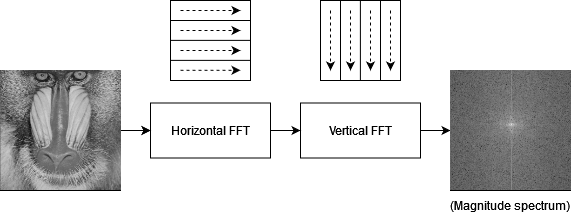
\includegraphics[width=0.75\textwidth]{tese/img/2d_fft.png}
    \caption{High-level illustration of horizontal and vertical passes}
    \label{fig:2d-fft}
\end{figure}

Additionally, the implementation of the 1D FFTs for every row and column is independent of the 2D FFT structure, hence, there is the freedom to use any of the discussed algorithms. In \autoref{chap:implementation-in-glsl}, we implement multiple FFT algorithms while reusing the same architecture of the horizontal and vertical passes.

% This logic applies to all complex to complex FFT implementations such as cuFFT without changing benchmark performance.
% \newline



% %TODO: 
% Talk about that microsoft paper which implements efficiently in HLSL

%%%%%%%%%%%%%%%%%%%%%%%%%%%%%%%%%%%%%%%%%%%%%%%%%%%%%%%%%%%%%%%%
%             Computation of the Fourier Transform             %
%%%%%%%%%%%%%%%%%%%%%%%%%%%%%%%%%%%%%%%%%%%%%%%%%%%%%%%%%%%%%%%%
% \chapter{Computation of the Fourier Transform}
% We introduce base knowledge to upgrade previous algorithms in many ways
% Stockham algorithm
% Radix-4 instead of Radix-2




%One could optimize the FFT by providing precomputed twiddle factors, or spare space for the output sequence by adopting an inplace FFT algorithm and all those factors influence the performance, evidently a balance must be established depending on the constraints for the FFT.

% \section{Natural order Cooley-Tukey} \label{subsec:natural-order-ct}

% % TODO: Paste here the lost paragraph

% Despite existing already really fast solutions for index bit reversal (\cite{prado2004new}), this \textit{shuffle} step still weights the algorithms with extra overhead. The natural order Cooley-Tukey FFT is a modification of the Cooley-Tukey algorithm that allows the removal of this step by computing the butterfly and reordering the elements per stage (\cite{OTFFTnoct}).

% \begin{figure}[h] 
%     \centering
%     \includegraphics[width=0.5\textwidth]{img/dif_elements_composition.png}
%     \caption{Chain of even and odd compositions over each stage for a natural order DIF}
%     \label{fig:dif-elements-composition}
% \end{figure}
% % Caption: Chain of compositions over each stage for a natural order DIF

% At the end of each stage the even and odd elements are composed in such a way that the elements will be in natural order at the end, as illustrated in \autoref{fig:dif-elements-composition}. This composition follows the indexing scheme described in \autoref{eq:nat_order_even_indexing}.

% % FIXME: Nao sei como ter isto tudo junto na mesma equacao
% \begin{equation} \label{eq:nat_order_even_indexing}
%     x[q + 2*p] = y[q + p] \\
% \end{equation}
% \begin{equation} \label{eq:nat_order_odd_indexing}
%     x[q + 2*p + 1] = y[q + p + m] \\
% \end{equation}

% Where $x$ and $y$ are alternated sequences for read and write over each stage, $q$ corresponds to the sub FFT offset in this stage, $p$ is the index of the sub \acrshort{fft} element shift for the current butterfly being computed, and finally $m$ corresponds to the size of the sub FFT divided by 2.

% Although this additional composition got rid of the bit reversal step in the Cooley-Tukey's algorithm, the computation is overloaded with more work for each stage, since first the algorithm computes the butterfly and then it reorders the elements every stage.

% This reordering after the butterfly may seem unnecessary, therefore we can use a new sequence and alternate between the two each stage, hence, providing this composition when we write the butterfly results. This is where the Stockham algorithm comes in.

% TODO: Rewrite better (maybe not very informative)
% We can also note that the composition of even and odd elements won't be necessary on the last stage of the DIF FFT since it will be a passthrough of the elements, so this is an unnecessary step, However, this algorithm is an intermediate step to make the Stockham algorithm more rational so there's no need to worry about this detail.



%%%%%%%%%%%%%%%%%%%%%%%%%%%%%%%%%%%%%%%%%%%%%%%%%%%%%%%%%%%%%%%%
%                  Implementation on the GPU                   %
%%%%%%%%%%%%%%%%%%%%%%%%%%%%%%%%%%%%%%%%%%%%%%%%%%%%%%%%%%%%%%%%
\chapter{Implementation in GLSL} \label{chap:implementation-in-glsl}

The previous chapters introduced and expanded upon \acrshort{fft} algorithms to compute the \acrshort{dft}, which provides enough background to back up the GPU implementations presented in this chapter.

As a result, in this chapter, we apply this background and implement these algorithms in \acrshort{glsl} compute shaders as a two-dimensional transform. 
%For this reason, we first describe how the 2D FFT is applied in \autoref{sec:2d-fourier-transform}. Furthermore, in \autoref{chap:implementation-in-glsl} is described in detail how we implemented and improved the algorithms to run on the GPU.


% \section{GLSL implementation} \label{sec:glsl-implementation}

The implementations were made using GLSL, a high-level shader language for graphics APIs such as OpenGL, and we used the compute pipeline from OpenGL to integrate an FFT implementation using compute shaders, which are general-purpose programmable shaders.

As there are many aspects that can impact performance, the implementation was an iterative process that required research and testing to compose a more suitable solution.
\newline
%One of the main targets was to keep the code generalized so that it could be used as the base for other implementations using FFTs with ease.


The next sections go into detail about the way every major iteration evolved into the next one and why there was the need to do it, starting with the Cooley-Tukey algorithm (\autoref{sec:ct-impl}) and then progressively improving to the Stockham algorithm (\autoref{sec:radix2-stockham} and \autoref{subsec:radix4-stockham})

% - [x] Brief about GLSL and the compute shaders used
% - [x]  Compute pipeline in GLSL
% - [x] Say it was an iterative process by applying, studying and testing

\section{Cooley-Tukey} \label{sec:ct-impl}

% Basic algorithm
% - iterative version
% - based on the dit described in state of art
% -

%FIXME: The beginning of this phrase is weird, rewrite
The GPU implementation took as a starting point the Cooley-Tukey algorithm since it is the most popular one with a time complexity of $O(N\log{(N)})$, and it is based on the iterative version adapted for parallel processors.

Since this implementation runs multiple threads in parallel we separated the reads and writes for each processor into two different buffers in memory due lack of order between processors, therefore, the declaration of two complex pingpong buffers.

\begin{lstlisting}[language=C, caption={Input buffer bindings}]
 layout (binding = 0, rg32f) uniform image2D pingpong0;
 layout (binding = 1, rg32f) uniform image2D pingpong1;
\end{lstlisting}

The read/write control for these buffers can be achieved with a flag variable \texttt{pingpong}.

Initially, this algorithm will work with a pass-per-stage approach, where a kernel is dispatched every stage, and since there is a synchronization step at the end of the pass it is granted that all the work groups have finished off writing to the buffer when a pass ends. This case holds up for both the horizontal and vertical FFT steps.

As a result, each kernel has the opportunity to work within every segment of the image, so the local threads can be dispatched with two dimensions, so each work group will have a total of 32 local threads, this number may vary depending on the GPU for optimal performance.

So an example dispatch group for this implementation could be $(fft\_width/8,fft\_height/8)$ work groups since 8 is the number of threads in the $y$ axis

By using GLSL there are some advantages to complex value operations since the addition and subtraction for vector types already have operator overloadings that work the same as in the complex domain. However, the multiplication works a bit differently so we need to provide an auxiliary function to abstract and support this operator.

\begin{lstlisting}[language=C, caption={Complex multiplication}]
 vec2 complex_mult(vec2 v0, vec2 v1) {
 	return vec2(v0.x * v1.x - v0.y * v1.y,
 				v0.x * v1.y + v0.y * v1.x);
 }
\end{lstlisting}

Due to the adoption of a different programming paradigm the FFT segment iteration loop doesn't exist such as in \autoref{alg:dit}, instead, the process identifiers are used to fetch the index of the butterflies they're gonna work on based on the work groups and threads dispatch setup, and this holds up for any implementation using compute shaders.

\begin{lstlisting}[language=C, caption={Invocation indices}]
 int line = int(gl_GlobalInvocationID.x);
 int column = int(gl_GlobalInvocationID.y);
\end{lstlisting}

Since this first approach is a dynamic implementation that invokes a pass-per-stage some stage control variables need to be fed into the shader in order to compute the correct butterfly index or control the butterfly process.

\begin{lstlisting}[language=C, caption={Uniform control variables}]
 uniform int pingpong;
 uniform int log_width;
 uniform int stage;
 uniform int fft_dir;
\end{lstlisting}

Effectively, we use these shader uniform input variables and obtain the actual index we are gonna use on the 1D FFT of the image.

\begin{lstlisting}[language=C, caption={FFT element index}]
 int group_size = 2 << stage;
 int shift = 1 << stage;
 
 int idx = (line % shift) + group_size * (line / shift);
\end{lstlisting}

To calculate the twiddle factor we use Euler's formula (\autoref{eq:euler}) and resort to the control variable \texttt{fft\_dir} to flip the twiddle factor for the inverse if we want to reuse this shader.

\begin{lstlisting}[language=C,caption={Euler's formula}]
 vec2 euler(float angle) {
     return vec2(cos(angle), sin(angle));
 }
 
 void main() {
     // ...
     vec2 w = euler(fft_dir * 2 * (M_PI / group_size) * ((idx % group_size) % shift));
     // ...
 }
\end{lstlisting}

% Explain butterfly
% - butterfly alternate read writes
Now with the computed twiddle factor, we may proceed to compute and store the Cooley-Tukey FFT butterfly, and that's where we need to control the reads and writes for each stage. Since the \texttt{pingpong} variable is toggled every pass invocation, it is used to choose with what texture we will use to look up the elements and which one to store into, and that is achieved with an if statement, just like it is used in \autoref{alg:stockham-dif}.

The butterfly computation itself is simply calculated as a Cooley-Tukey DIT butterfly as presented in \autoref{subsec:radix-2-decimation-in-time-fft}.

\begin{lstlisting}[language=C,caption={Computation of the Cooley-Tukey butterfly}]
 if (pingpong == 0) {
     // Read
     a = imageLoad(pingpong0, ivec2(idx, column)).rg;
     b = imageLoad(pingpong0, ivec2(idx + shift, column)).rg;

     // Compute and store
     vec2 wb = complex_mult(w, b);
     vec2 raux = a + wb;
     imageStore(pingpong1, ivec2(idx, column), vec4(raux, 0, 0));
     raux = a - wb;
     imageStore(pingpong1, ivec2(idx + shift, column), vec4(raux, 0, 0));
 }
 else {
     // Read
     a = imageLoad(pingpong1, ivec2(idx, column)).rg;
     b = imageLoad(pingpong1, ivec2(idx + shift, column)).rg;
     
     // Compute and store
     vec2 wb = complex_mult(w, b);
     vec2 raux = a + wb;
     imageStore(pingpong0, ivec2(idx, column), vec4(raux,0,0));    
     raux = a - wb;
     imageStore(pingpong0, ivec2(idx + shift, column), vec4(raux,0,0));
 }
\end{lstlisting}

Finally, there is only one step missing, the bit reversal of indices to have a natural order result. A \texttt{bit\_reverse} function could be easily defined, However, there's already a GLSL alternative which is \texttt{bitfieldReverse} together with \texttt{bitfieldExtract} (\cite{kessenich4opengl}).

% Despite not having a noticeable performance hit, it is good practice to use GLSL predefined functions and operators since they might be optimized for that specific device hardware, and using these functions instead of a handmade implementation reduces the kernel size significantly by about approximately 400 bytes (tested using \textit{glslang}) since they are reusable functions. 

\begin{lstlisting}[language=C,caption={Auxiliary function that takes advantage of GLSL's predefined utilities}]
 int bit_reverse(int k) {
     uint br = bitfieldReverse(k);
     return int(bitfieldExtract(br, 32 - log_width, log_width));
 }
\end{lstlisting}

% - butterfly initial bit reverse on first stage
This auxiliary function will be conditionally used inside the branching if statement for alternating read/writes to be only applied on the first stage of transform both for the possible values of \texttt{pingpong == 0} and \texttt{pingpong == 1}, since the vertical pass might start reading on the first pingpong buffer. This is not the case for the horizontal pass, it is ensured that the first stage will always read from \texttt{pingpong0} reinforcing that the bit reverse branching when \texttt{pingpong == 0} is disposable.

\begin{lstlisting}[language=C,caption={Computation of the Cooley-Tukey butterfly with bit reversal}]
 if (pingpong == 0) {
     if (stage == 0) {
         a = imageLoad(pingpong0, ivec2(bit_reverse(idx), column)).rg;
         b = imageLoad(pingpong0, ivec2(bit_reverse(idx + shift), column)).rg;
     }
     else {
         a = imageLoad(pingpong0, ivec2(idx, column)).rg;
         b = imageLoad(pingpong0, ivec2(idx + shift, column)).rg;
     }

     // ... Compute and store results
 }
 else {
     a = imageLoad(pingpong1, ivec2(idx, column)).rg;
     b = imageLoad(pingpong1, ivec2(idx + shift, column)).rg;

     // ... Compute and store results
 }
\end{lstlisting}

%We can already see some branching in this code that might not be desirable.
% Cooley-Tukey

% Initial implementation model
% - [x]Read write requirements
% - [x] Per stage synchronization (multiple submissions)
% - [ ] 2D Work dispatch (with illustration)

% - [x] Vector type operations
% - [x] Mention to use GLSL bitreverse instead of manual implementation (perhaps no noticeable performance but the kernel size reduces significantly)
% - pass-per-stage
%     - The way it is dispatched and why it is made that way
% - Updating to all stages in a single pass
%     - One problem of this is the synchronization between threads
%     - And by using only 1 pass for all stages there's a big difference, the implementation can be static for the size, so there's no branching associated, with that the pingpong variable now is constexpr so the compiler optimizes the kernel execution to inline the ifstatement and the while loop
% - Reference somewhere with loop unroll glsl version




With all these steps aggregated, the shader for the horizontal pass of this FFT DIT Cooley-Tukey implementation is presented in \autoref{lst:glsl-radix2-ct-stage-horizontal}, see \autoref{apdx:glsl-fft}.


% TODO: Mention this normalization in the 2D
For the vertical pass shader, there is, however, one extra multiplication by \texttt{mult\_factor} in the butterfly results for the last stage when the pass is inverse. This corresponds to the normalization of the multidimensional transform similar to the normalization in the inverse DFT in \autoref{eq:discrete-fourier-transform}, this is demonstrated in \autoref{lst:glsl-radix2-ct-stage-vertical}.

% We can already see in \autoref{lst:glsl-ct-stage-vetical} the above code a lot of branching that might be undesirable on the GPU  ... % TODO: Reference that thing where a warp branching has a huge performance hit due to the way it is implemented

\subsection{All stages in one pass} \label{subsec:all-stages-in-one-pass}

The previous implementation demonstrates a generic 2D FFT that may be reused for multiple FFT sizes, However, this comes at a cost of efficiency when it comes to the synchronization of the of the stage itself, moreover, it requires use multiple uniform variables for control of the FFT that are transferred between CPU and GPU when there are updates in between stages.
\newline

% NOTE: Uncertain if the 'kernel-wise' is a good way to say it
The ideal solution here is to port this implementation synchronization step to be kernel-wise and this detail changes how the code is structured and how it may be dispatched.


% TODO: maybe list some references here "a lot of literature on behalf of GPU compute execution synchronization"
There is a lot of literature on behalf of GPU compute execution synchronization (\cite{stuart2011efficient}). In our case we make use of execution barriers that synchronize all the threads within a work group (\cite{kessenich4opengl}).

The current grouping of threads doesn't allow the use of these barrier synchronizations since the computation of one-dimensional FFT is distributed between multiple work groups, thus, using a call to \texttt{barrier()} inside the kernel wouldn't fix the race conditions of several segments of the image. We could, however, change the setup of these work groups in such a way that each 1D FFT threads fit in one work group as illustrated in \autoref{fig:invocation-space}. 


\begin{figure}[h] 
    \begin{subfigure}{.5\textwidth}
        \centering
        \includegraphics[width=0.8\textwidth]{tese/img/inv_space_2d.png}
    \end{subfigure}
    \begin{subfigure}{.5\textwidth}
        \centering
        \includegraphics[width=0.8\textwidth]{tese/img/inv_space_1d.png}
    \end{subfigure}
    % FIXME: Maybe this name is not very great
    \caption{Difference in invocation spaces for size 256 FFT to allow barrier synchronization between local threads}
    \label{fig:invocation-space}
\end{figure}

By restricting the invocation space to be only one dimensional we grant the possibility to use the barrier correctly but at the cost of resizability, the work group's local size must now be restricted to half the size of the FFT. This restriction does not affect our results, where the tests were performed on images with a relatively small size. The GPU is extremely parallel hardware, therefore, it is better to dispatch smaller programs with more instances than overloading local threads in a work group to decrease its.
\newline 

When fitting all stages in one kernel, the algorithm stays the same but we provide all information needed, such as the size and log size of the FFT for the compiler to be able to unroll the loop, since the for loop feature in GLSL requires to be used with constant expressions that allow the loop to be inlined in the compiled code.
\newline 

\begin{lstlisting}[language=C,caption={Unique pass structure for Cooley-Tukey}]
#define FFT_SIZE 256
#define LOG_SIZE 8

layout (local_size_x = FFT_SIZE/2, local_size_y = 1) in;

layout (binding = 0, rg32f) uniform image2D pingpong0;
layout (binding = 1, rg32f) uniform image2D pingpong1;
uniform int fft_dir;
// ... Auxiliar functions

void main() {
    // ...
    int pingpong = 0;
    
    for(int stage = 0; stage < LOG_SIZE; ++stage) {
        int group_size = 2 << stage;
        int shift = 1 << stage;

        vec2 a, b;
        int idx = (line % shift) + group_size * (line / shift);
        vec2 w = euler(fft_dir * 2 * (M_PI / group_size) * ((idx % group_size) % shift));
        // ... Perform butterflies

        pingpong = (pingpong + 1) % 2;
        barrier();
    }
}
\end{lstlisting}

Aside from the variable \texttt{fft\_dir} that allows the usage of this pass for the inverse, all needed data for the FFT lives inside the code, hence, there are more opportunities for optimization when the kernel is compiled since most data is within the code itself. For full code for horizontal and vertical passes see \autoref{apdx:glsl-fft}.

% Updating to all stages in a single pass %
% - One problem of the previous is the synchronization between threads and multiple input variables for control that update on the cpu.
% - For this we need to sync inside fft and we dont have a way to arbitrarly sync between work groups but we can sync between local threads
% - Dispatch settings may be changed to allow an implementation to sync the stage between reads and writes for each one dimensional FFT
%   - Image that represents the before and after of the dispatch architecture
% - Pros and const of this way of dispatching work groups
%   - Cons: there is less immediate control over how many threads we want in each work group since we need as many as FFT_SIZE / 2.
% - Mention we tested multiple butterflies and that doesn't improve the performance since the kernel wants to finish as soon as possible and the work group size isn't the problem here
% ====================================== %

% - And by using only 1 pass for all stages there's a big difference, the implementation can be static for the size, so there's no branching associated, with that the pingpong variable now is constant expression so the compiler optimizes the kernel execution to inline the if statement and the while loop
% - Reference somewhere with loop unroll glsl version

\section{Radix-2 Stockham} \label{sec:radix2-stockham}

Since we wanted to get rid of the bit reversal permutation in the shader code, we implemented the Stockham algorithm (see \autoref{sec:stockham-algorithm}). What differs from the previous code is mainly the reordering of the elements when writing the results of the butterfly. %It is also important to note that this algorithm is in DIF instead of DIT like the previous ones.

Note that this algorithm is in DIF instead of DIT like the previous ones, although this change does not have a performance implication.
\newline


When performing the butterfly in \autoref{lst:stockham-reordering}  we read the elements from the image according to the thread identifier, however, we store it in such a way that the output has its elements in natural order (see \autoref{alg:stockham-dif}).

\begin{lstlisting}[language=C, caption={Radix-2 Stockham DIF}, label={lst:stockham-reordering}]
for(int stage = 0; stage < LOG_SIZE; ++stage) {
    int n = 1 << (LOG_SIZE - stage); // group_size
    int m = n >> 1; // shift
    int s = 1 << stage;

    int p = line / s;
    int q = line % s;
    vec2 wp = euler(fft_dir * 2 * (M_PI / n) * p);
    
    if(pingpong == 0) {
        vec2 a = imageLoad(pingpong0, ivec2(q + s*(p + 0), column)).rg;
        vec2 b = imageLoad(pingpong0, ivec2(q + s*(p + m), column)).rg;

        vec2 res = (a + b);
        imageStore(pingpong1, ivec2(q + s*(2*p + 0), column), vec4(res,0,0));
        res = complex_mult(wp,(a - b));
        imageStore(pingpong1, ivec2(q + s*(2*p + 1), column), vec4(res,0,0));
    }
    else {
        // ... Read pingpong1, write pingpong0
    }
    
    // ... Sync
}
\end{lstlisting}

Consequently, we got rid of the conditional read with bit reversed index, and the compute shader code for the horizontal \autoref{lst:glsl-radix2-stockham-horizontal} and vertical passes \autoref{lst:glsl-radix2-stockham-vertical} got simpler as a result of this.

\section{Radix-4 Stockham} \label{subsec:radix4-stockham}

In \autoref{sec:radix4-instead-of-radix2} we introduced how higher radix factorizations could improve the performance with the cost of size constraints, hence, here we change the code with ease to implement the radix-4 factorization described previously.
\newline

First, we update the stage control variables and compute the multiple twiddle factors used in the radix-4 butterfly. Note that now the for loop only iterates $\log{(N)}/2$ times and the number of local threads is reduced by half.

\begin{lstlisting}[language=C, caption={Radix-4 Stockham stage control variables}, label={lst:radaix4-stockham-control-vars}]
#define FFT_SIZE 256
#define LOG_SIZE 8 // log2(FFT_SIZE)
#define HALF_LOG_SIZE 4 // log2(FFT_SIZE) / 2

layout (local_size_x = FFT_SIZE/4, local_size_y = 1) in;

// ...

void main() {
    // ...

    for(int stage = 0; stage < HALF_LOG_SIZE; ++stage) {
        int n = 1 << (HALF_LOG_SIZE - stage)*2;
        int s = 1 << stage*2;

        int n0 = 0;
        int n1 = n/4;
        int n2 = n/2;
        int n3 = n1 + n2;

        int p = line / s; 
        int q = line % s;

        vec2 w1p = euler(2*(M_PI / n) * p * fft_dir);
        vec2 w2p = complex_mult(w1p,w1p);
        vec2 w3p = complex_mult(w1p,w2p);

        // ... Radix-4 butterfly
    }
}
\end{lstlisting}

Then, we compute the radix-4 butterfly and store the results in natural order, as described in \autoref{fig:radix4-dragonfly}.
\newline 

\begin{lstlisting}[language=C, caption={Radix-4 Stockham butterfly}, label={lst:radix4-stockham-dragonfly}]
if(pingpong == 0) {
    vec2 a = imageLoad(pingpong0, ivec2(q + s*(p + n0), column)).rg;
    vec2 b = imageLoad(pingpong0, ivec2(q + s*(p + n1), column)).rg;
    vec2 c = imageLoad(pingpong0, ivec2(q + s*(p + n2), column)).rg;
    vec2 d = imageLoad(pingpong0, ivec2(q + s*(p + n3), column)).rg;

    vec2 apc = a + c;
    vec2 amc = a - c;
    vec2 bpd = b + d;
    vec2 jbmd = complex_mult(vec2(0,1), b - d);

    imageStore(pingpong1, ivec2(q + s*(4*p + 0), column), vec4(apc + bpd, 0,0));
    imageStore(pingpong1, ivec2(q + s*(4*p + 1), column), vec4(complex_mult(w1p, amc - jbmd), 0,0));
    imageStore(pingpong1, ivec2(q + s*(4*p + 2), column), vec4(complex_mult(w2p, apc - bpd ), 0,0));
    imageStore(pingpong1, ivec2(q + s*(4*p + 3), column), vec4(complex_mult(w3p, amc + jbmd), 0,0));
}
else {
    // ...
}
\end{lstlisting}

We take advantage of branchless programming to flip the signal of the butterfly to avoid unnecessary if statements for the inverse.

\begin{lstlisting}[language=C, caption={Radix-4 Stockham dragonfly inverse arithmetic}, label={lst:radix4-stockham-dragonfly-arithmetic}]
imageStore(pingpong1, ivec2(q + s*(4*p + 0), column), vec4(apc + bpd, 0,0));
imageStore(pingpong1, ivec2(q + s*(4*p + 1), column), vec4(complex_mult(w1p, amc + jbmd*fft_dir), 0,0));
imageStore(pingpong1, ivec2(q + s*(4*p + 2), column), vec4(complex_mult(w2p, apc - bpd ), 0,0));
imageStore(pingpong1, ivec2(q + s*(4*p + 3), column), vec4(complex_mult(w3p, amc - jbmd*fft_dir), 0,0));
\end{lstlisting}


With these changes, we now have the radix-4 Stockham shader complete (see \autoref{lst:glsl-radix4-stockham-horizontal} and \autoref{lst:glsl-radix4-stockham-vertical}).
\newline 

Furthermore, we may expand the implementation of this radix-4 compute shader, in such a way that it supports power of $2$ sizes instead of just power of $4$. For example, when a power of 2 size input is used in the radix-4 Stockham algorithm it performs half of $\log{(N)}$ stages, meaning that it will miss one final stage for a sub-transform with a size that is not multiple of $4$. In this final stage, we may apply the radix-2 Stockham algorithm stage as an additional step to grant support for power of 2 sizes.

% - On the compute shader for the radix-4 Stockham we add the final stage
% - No twiddle factor needed, due to p == 0
% - Perform 2 raadix-2 butterflies due to local_size_x = FFT_SIZE/4 
% - Code for the last stage
With this said, at the end of the compute shader in the radix-4 implementation we add a conditional last step implementing the radix-2 Stockham stage butterflies. Likewise, this stage corresponds to the same code as in \autoref{sec:radix2-stockham}, but partially more hardcoded for the last stage. For this reason, the presented code doesn't use a twiddle factor, since it will always correspond to $1$ due to parameter $p$ being equal to $0$ for the last stage.

Finally, since we only have $FFT\_SIZE/4$ local threads, therefore, $2$ butterflies need to be computed at a time, as demonstrated in \autoref{lst:radix4-stockham-radix2-stage}.

\begin{lstlisting}[language=C, caption={Radix-2 stage for the radix-4 Stockham code}, label={lst:radix4-stockham-radix2-stage}]
#define FFT_SIZE 512
#define LOG_SIZE 9 // log2(FFT_SIZE)
#define HALF_LOG_SIZE 4 // log2(FFT_SIZE / 2) / 2

int main() {
    // ... radix-4 Stockham stages

    if(LOG_SIZE % 2 == 1) {
        int s = FFT_SIZE >> 1;
        int q = 2*line;

        if(pingpong == 0) {
            vec2 a = imageLoad(pingpong0, ivec2(q + 0, column)).rg;
            vec2 b = imageLoad(pingpong0, ivec2(q + s, column)).rg;
            imageStore(pingpong1, ivec2(q + 0, column), vec4(a + b, 0,0));
            imageStore(pingpong1, ivec2(q + s, column), vec4(a - b, 0,0));

            q = 2*line + 1;
            a = imageLoad(pingpong0, ivec2(q + 0, column)).rg;
            b = imageLoad(pingpong0, ivec2(q + s, column)).rg;
            imageStore(pingpong1, ivec2(q + 0, column), vec4(a + b, 0,0));
            imageStore(pingpong1, ivec2(q + s, column), vec4(a - b, 0,0));
        }
        else {
            vec2 a = imageLoad(pingpong1, ivec2(q + 0, column)).rg;
            vec2 b = imageLoad(pingpong1, ivec2(q + s, column)).rg;
            imageStore(pingpong0, ivec2(q + 0, column), vec4(a + b, 0,0));
            imageStore(pingpong0, ivec2(q + s, column), vec4(a - b, 0,0));

            q = 2*line + 1;
            a = imageLoad(pingpong1, ivec2(q + 0, column)).rg;
            b = imageLoad(pingpong1, ivec2(q + s, column)).rg;
            imageStore(pingpong0, ivec2(q + 0, column), vec4(a + b, 0,0));
            imageStore(pingpong0, ivec2(q + s, column), vec4(a - b, 0,0));
        }
    }
}
\end{lstlisting}

%Likewise, 




% - The Inverse required mmore changes to the butterfly operation, but we use branchless programming to avoid unnecessary if statements

% - We may use simple multiplication arithmethic to flip the operator according to the fft direction
% - Explain what is branchless programming and how it may affect the code and how it may not affect this code
% - Information  obtained directly from compiling source code with a shader compiler to intermediate representation
% - Any shader compiler strips down every piece of the kernel and tries to apply optimizations to most operations
% TODO: Testing inlined loop vs the code provided


% - Matrix transposition mention, and that the results may not be better



%%%%%%%%%%%%%%%%%%%%%%%%%%%%%%%%%%%%%%%%%%%%%%%%%%%%%%%%%%%%%%%%
%                   Analysis and Comparison                    %
%%%%%%%%%%%%%%%%%%%%%%%%%%%%%%%%%%%%%%%%%%%%%%%%%%%%%%%%%%%%%%%%
\chapter{Analysis and Comparison} \label{chap:analysis-and-comparison}
% - Explain whats this chapter about
% - First we'll make the comparison with same algorithms in CUDA
% - Then we'll talk about popular implementations like cuFFT and the merit they have to compare them with our implementation in GLSL 

Finally, in this chapter, an evaluation of the explored implementations and improvements is provided followed by an empirical analysis based on the results and tests done. 

To establish a reference point on the results provided, we used \acrshort{cufft} which is the \acrshort{cuda} Fast Fourier Transform library from NVIDIA.

%Additionally, to deepen the analysis, this chapter also delivers an equivalent comparison of the researched algorithms applied to a different \acrshort{gpgpu} compute framework such as \acrshort{cuda}. %To convey a


%%%%%%%%%%%%%%%%%%%%%%%%%%%%%%%%%%%%%%%%%%%%%%%%%%%%%%%%%%%%%%%%

\section{cuFFT} \label{sec:cufft}
% TODO:
% - What it is
% - Pros and cons (NVIDIA only)
% - Sample code for in and out of place implementations
% - It selects the best algorithm and properties of the fft to achieve best performance
% - The performance of cufft is used as a reference for the difference of the other benchmarks
% - Conditions used for the conmparison

The cuFFT library is the NVIDIA framework designed to provide high performance \acrshort{fft} exclusively on its own GPUs that supports a wide range of \acrshort{fft} inputs and settings that compute \acrshort{fft}s efficiently on NVIDIA GPUs.

It has been proven multiple times that cuFFT is one of the fastest available tools for computing FFT such as in \cite{sorman2016comparison} and other resources.

The \acrshort{cufft} library is acknowledged as one of the most efficient FFT GPU frameworks for the flexibility it provides and it is "\textit{de-facto a standard GPU
implementation for developers using CUDA}" (\cite{stvrelak2018performance}). Furthermore, it offers all kinds of settings needed for most use cases, such as multidimensional transforms, complex and real-valued input and output, support for half, single, and double floating point precision, execution of multiple transforms simultaneously, and finally, since all this is implemented using \acrshort{cuda} we can take advantage of streamed execution, enabling asynchronous computation and data movement.

Unfortunately, as mentioned before the main downside of \acrshort{cufft} is the unavailability of this library for GPUs from other vendors.
\newline

The \acrshort{cufft} library uses algorithms highly optimized for input sizes that can be written in the form $2^a \times 3^b \times 5^c \times 7^d$, so it factorizes the input size to allow arbitrary-sized FFT sequences. Furthermore, sizes with lower prime factors have better performance than higher prime factors (\cite{nvidiacufft}), thus power of $2$ sizes have the best performance overall.
\newline

To use the results of the \acrshort{cufft} library as a reference point, we need to establish equivalent conditions to that of the GLSL implementations:

\begin{itemize}
    \item Out-of-place 2D FFT, the input buffer is different from the output buffer;
    \item Power of 2 input sizes, such as 128, 256, 512, and 1024;
    \item Complex to complex FFT, input and output buffer are complex-valued;
    \item The benchmarks are average milliseconds of multiple executions, however, the first dispatch is not taken into account since  takes extra time to set up things on the \acrshort{gpu}.
\end{itemize}

The results of the cuFFT out-of-place benchmarks are presented in \autoref{fig:cufft-glsl-benchmarks}.

\section{GLSL implementation results} \label{sec:glsl-implementation-results}
% - Compare all implementations from section 5.3.2
% - List of benchmark conditions
% - Details reasons why the results are this way (reference here the graphs)
%   - First why the pass-per-stage approach has worst performance overall (include app frame count)
%   - Discuss Radix-2 Cooley-Tukey vs Radix-2 Stockham
%   - Discuss how Radix-4 improves the Radix-2
%     - Computes 4 values at a time
%     - Less synchronization between Workgroup
%     - Less stages so less synchronization -
%     - Higher or lower sized kernel (comparing to radix-2)

The implementations discussed in \autoref{chap:implementation-in-glsl} were studied and benchmarks were made to come to a conclusion about the advantages and disadvantages of using each one and how do they perform. With this in mind, we prepared an interactive test environment using Nau 3D engine (\cite{nau3d}) and profiled it using an internal pass profiler.

The benchmark results in this section were tested with the following hardware and software configurations:

\begin{itemize} \label{itm:benchmark-conditions}
    \item \textbf{CPU:} Intel(R) Core(TM) i7-8750H @ 2.20GHz;
    \item \textbf{GPU:} NVIDIA GeForce GTX 1050 Ti Max-Q;
    \item \textbf{NVIDIA driver:} 511.65;
    \item \textbf{CUDA version:}  V11.6.124;
    \item \textbf{GLSL version:}  4.60.
\end{itemize}

% STAGE PASS VS UNIQUE PASS
In \autoref{subsec:all-stages-in-one-pass} we discussed how the implementation would benefit by having a unique pass that synchronized by stage instead of dispatching multiple stage passes. Accordingly, to prove this, we evaluated the difference between the Cooley-Tukey algorithm in the unique pass and in a stage-per-pass approach. Hence, in \autoref{fig:stage-pass-vs-unique-pass} are presented the CPU and GPU results of the benchmarks for this test case. The GPU time corresponds to the total time spent in the GPU executing the compute shader.

These benchmarks were tested in Nau3D, a generic 3D rendering engine, therefore, the CPU side of the stage-per-pass implementation takes into account the execution of a \textit{Lua} script to update the state and control variables at the end of each stage. For this reason, the CPU time besides the preparation of the compute dispatch also includes some overhead for using this \textit{Lua} script.

\begin{figure}[H] 
    \begin{subfigure}{.5\textwidth}
        \centering
        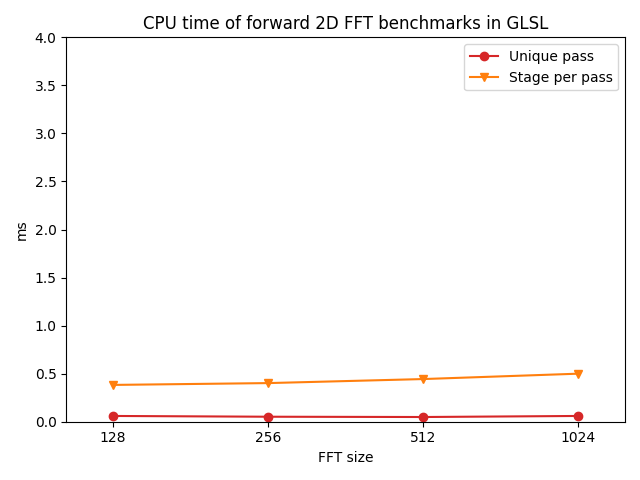
\includegraphics[width=0.9\textwidth]{img/results/glsl_stage_pass_vs_unique_pass_cpu.png}
    \end{subfigure}
    \begin{subfigure}{.5\textwidth}
        \centering
        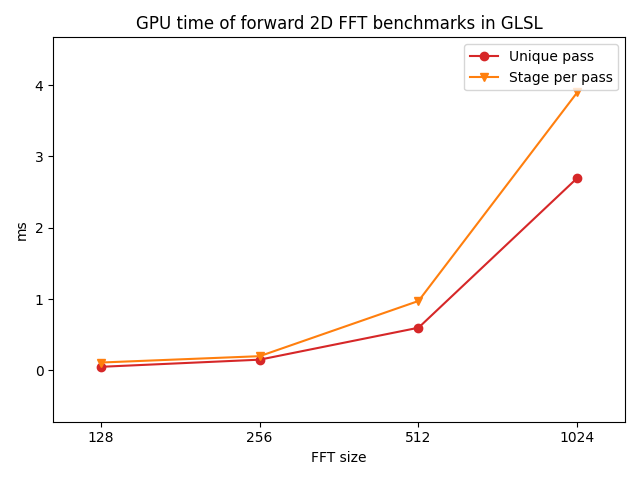
\includegraphics[width=0.9\textwidth]{img/results/glsl_stage_pass_vs_unique_pass_gpu.png}
    \end{subfigure}
    \caption{CPU and GPU time of 2D forward FFT using stage per pass approach and unique pass for the Radix-2 Cooley-Tukey algorithm}
    \label{fig:stage-pass-vs-unique-pass}
\end{figure}


% - Analisar os resultados
% - In the unique pass, the work occurs exclusively on the GPU therefore the CPU time is mostly constant
% - Therefore in the next comparisons this stage-per.pass approach (Já nao vai estar presente nas restantes comparações)


The results in \autoref{fig:stage-pass-vs-unique-pass} demonstrate the approximate expected overhead of using the stage-per-pass in an application. Since there is a need for the update of the following stages, the implementation synchronizes with the GPU immediately over each stage, however, the compute shader is reusable, therefore, the same shader module can be used for multiple sizes. In contrast, the CPU time of the unique pass kernel is mostly constant and this approach is optimized for its own size so most calculations are inlined by the GLSL compiler. The stage synchronization is kept inside the GPU until the kernel completes the execution. Since this type of synchronization is on the work group level, much fewer actors are involved in the synchronization step. In addition, these actors only correspond to the 1D FFT region of each row/column and not the entire 2D FFT.

Due to the difference in the performance of these two approaches, the following comparisons will exclusively correspond to unique pass implementations of the investigated algorithms.
\newline


% FIXME: Don't know how to blend the comparisons 
As we can see in \autoref{fig:cufft-glsl-benchmarks} we plot the performance of the benchmarks of cuFFT and the unique pass algorithms in GLSL. These implementations are the single-pass approaches of the discussed algorithms in \autoref{chap:implementation-in-glsl}. Based on the findings of these benchmarks, the GLSL radix-2 implementation of the Stockham algorithm has an overall better performance comparing it to the Cooley-Tukey version. Additionally, it was also implemented with a smaller kernel. Consequently, this happens due to the removal of the data reordering process of the bit reversal done in the Cooley-Tukey version only in the first stage. Effectively, this change improves the results consistently within the test size ranges. %, however, it is worth noting that the Stockham algorithm has worst data access locality than the Cooley-Tukey algorithm since it accesses data arbitrarily within the FFT instead of performing the sorting right away, therefore, these results may not hold this way for larger sizes.


%As we can see in \autoref{fig:cufft-glsl-benchmarks} the GLSL radix-2 implementation of the Stockham algorithm has overall better performance comparing it to the Cooley-Tukey version. This happens due to the removal of the data reordering process of the bit reversal done in the Cooley-Tukey version only on the first stage. Effectively, this change improves the results consistently within the test size ranges, however, it is worth noting that the Stockham algorithm has worst data access locality than the Cooley-Tukey algorithm since it accesses data arbitrarily within the FFT instead of performing the sorting right away, therefore, these results may not hold this way for larger sizes.

\begin{figure}[h!] 
    \centering
    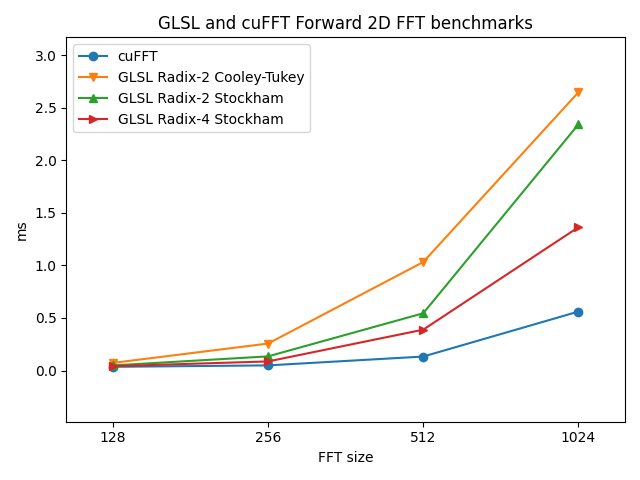
\includegraphics[width=0.65\textwidth]{img/results/cufft_glsl_benchmarks.png}
    \caption{Forward 2D FFT benchmarks in milliseconds of out-of-place cuFFT and unique pass algorithms in GLSL}
    \label{fig:cufft-glsl-benchmarks}
\end{figure}

% FIXME: 'halfway close'? nao tenho a certeza se isto é um bom ingles
Undoubtedly, the results that come closer to the cuFFT are the ones of the radix-4 Stockham. It drastically improved the performance halfway close to the cuFFT, as presented in \autoref{fig:cufft-glsl-benchmarks}. Yet, the complexity of the shader code was sharply increased, not only due to the higher radix alternative but also due to the additional support step in the last stage for the power of $2$ sizes.

By choosing a radix-4 approach the number of stages reduces to half but with a lot more complex operations per dragonfly on each stage. Since this dragonfly represents the operations required in an equivalent radix-2 Stockham factorization. Although the work complexity remains the same, there are much fewer barrier synchronization events and radix-4 iterations perform the work of two radix-2 iterations with only one memory access.

For each stage there's a synchronization barrier in each local thread inside a work group, so fewer stages means fewer sync points, hence, compensating for the 70\% kernel size increase of the radix-4 version.

% MULTIPLE BUTTERFLIES PER LOCAL THREAD
% It is also worth noting, in our benchmarks we tested the possibility to integrate multiple butterflies per threads in hope that there was a threshold on the number of local threads that would compensate the workload per kernel for less threads in the synchronization step. However, this didn't happen, and for all implementations introducing multiple butterflies per thread and reducing the number of threads. This approach didn't improve the performance overall, so the results of this testing are presented in \autoref{fig:glsl-multiple-butterflies} for the Radix-2 Stockham algorithm. We can conclude that the compute shaders can handle well high threads work groups, therefore less work per kernel is preferred instead of lesser threads per work group.

% \begin{figure}[H] 
%     \centering
%     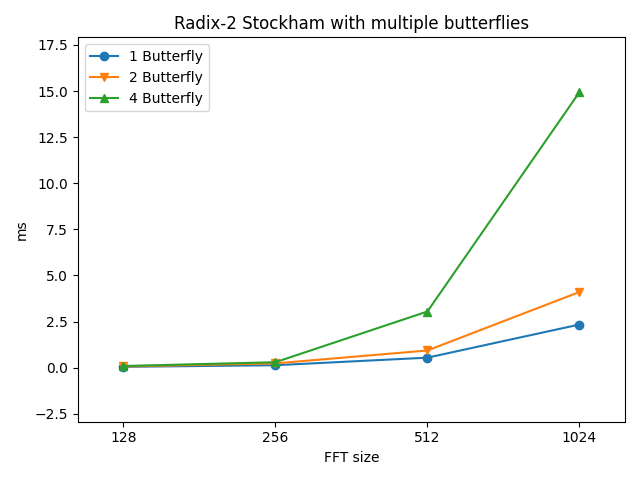
\includegraphics[width=0.65\textwidth]{img/results/glsl_multiple_butterflies.png}
%     \caption{2D FFT benchmarks in milliseconds of GLSL Radix-2 Stockham with multiple butterflies per local threads}
%     \label{fig:glsl-multiple-butterflies}
% \end{figure}



% MULTIPLE FFTs USING VEC4
In the context of the same need for multiple FFTs, we reach a point where we need to batch executions together for cuFFT. While this can also be achieved using our GLSL implementations, we can take a step further on the usage of the same pass for double the FFTs. Accordingly, we adapted the radix-4 Stockham implementation to use \texttt{vec4} instead of \texttt{vec2} for the elements of the input and output buffers.

% How we changed the code in GLSL
Code integrity is conserved since changing to \texttt{vec4} does not change operators in the compute kernel. 

% Explain how we instantiated multiple batched (2 in this case) for cuFFT
To compare with an equivalent, the computation in cuFFT used a special setup of a 2D FFT plan to compute with a batch size of $2$. The cuFFT framework doesn't have an explicit setup for multiple transforms in the same kernel, hence, we use batched execution for comparison.

\begin{figure}[H] 
    \centering
    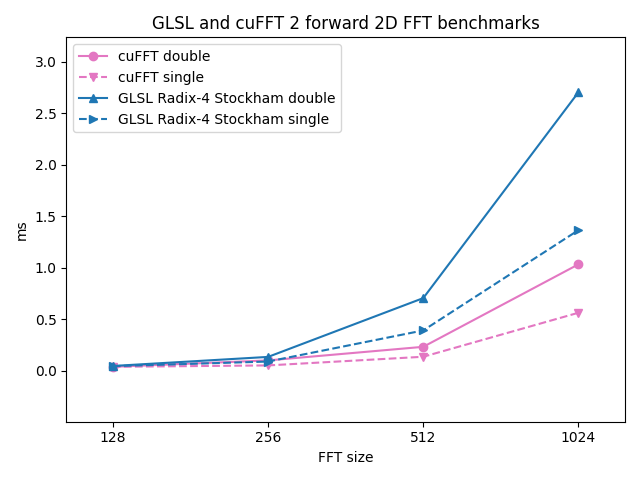
\includegraphics[width=0.6\textwidth]{tese/img/results/cufft_glsl_multiple_fft_benchmarks.png}
    \caption{Forward 2D FFT benchmarks of double the transforms in milliseconds of out-of-place cuFFT and radix-4 Stockham GLSL}
    \label{fig:cufft-glsl-multiple-fft-benchmarks}
\end{figure}

% IN CORRECTION STATE: As we can see in \autoref{fig:cufft-glsl-multiple-fft-benchmarks} the double FFTs have a near linear increase with some benefits for specific sizes. To analyze the difference of single FFT performance in this double FFT approach we present in \autoref{tab:cufft-glsl-single-double} the percentage of performance increase per transform comparing to the results in \autoref{fig:cufft-glsl-benchmarks}.

In table \autoref{tab:cufft-glsl-single-double}, the benchmarks of \autoref{fig:cufft-glsl-multiple-fft-benchmarks} are presented together with the results of calculating a single transform in one step. To analyze the potential gain that the implementation with twice the transforms gives, we also present the percentage of the performance gain per individual FFT.


\begin{table}[H]
    \centering
    \begin{tabular}{|cc|c|c|c|c|}
    \hline
    \multicolumn{2}{|c|}{\textbf{Sizes}}                                                        & \textbf{128}     & \textbf{256}     & \textbf{512}     & \textbf{1024}   \\ \hline
    \multicolumn{1}{|c|}{\multirow{3}{*}{\textbf{cuFFT}}}                 & Single FFT          & 0.035   & 0.049   & 0.133   & 0.560  \\ \cline{2-6} 
    \multicolumn{1}{|c|}{}                                                & Double FFT          & 0.038   & 0.098   & 0.23    & 1.032  \\ \cline{2-6} 
    \multicolumn{1}{|c|}{}                                                & Gain per single FFT & 45.71\% & 0.0\%   & 13.53\% & 7.85\% \\ \hline
    \multicolumn{1}{|c|}{\multirow{3}{*}{\textbf{GLSL radix-4 Stockham}}} & Single FFT          & 0.042   & 0.087   & 0.389   & 1.363  \\ \cline{2-6} 
    \multicolumn{1}{|c|}{}                                                & Double FFT          & 0.044   & 0.132   & 0.704   & 2.702  \\ \cline{2-6} 
    \multicolumn{1}{|c|}{}                                                & Gain per single FFT & 47.61\% & 24.13\% & 9.51\%  & 0.88\% \\ \hline
    \end{tabular}
    \caption{Benchmarks of the Forward 2D FFT for cuFFT and GLSL radix-4 Stockham for single and double transforms in the same pass, together with the percentage of gain over individual transforms.}
    %
    %Forward 2D FFT benchmarks of double the transforms in milliseconds of out-of-place cuFFT and radix-4 Stockham GLSL
    \label{tab:cufft-glsl-single-double}
\end{table}


As a result, we can clearly notice a larger gain for size 128 inputs, both for cuFFT and for GLSL. From there, the gain for the rest of the tested sizes is notably smaller, the most relevant gain being that of inputs of size $256$ for GLSL since cuFFT did not show any difference to twice the time of a single FFT for this input size. Finally, for input sizes 512 and 1024 the cuFFT batched execution demonstrated a valuable gain while the GLSL one continued to decline.

Overall, we can conclude that it is worth including multiple FFTs in the same \textit{pass} for the tested sizes when multiple independent transforms are necessary. \newline

% Despite the size $128$, the results don't correspond to huge differences and the sizes above $128$ have a close to linear increase for the double FFT. However, for the size $256$, the GLSL implementation gets closer to the cuFFT due to having a more beneficial double FFT performance difference.


%With the presented results, a GLSL programmer might want to implement this radix-4 Stockham algorithm on the GPU. Alternatively, for a simpler implementation, radix-2 suits best with a good trade-off of simplicity over performance.

With the presented results, we can clearly notice better performance on the GPU regarding the implementation in GLSL of radix-4 Stockham with a unique pass approach that reduces the number of synchronization stages and calculates per dragonfly the equivalent $2$ butterflies of two stages of radix-2 Stockham.

\section{Case of study} \label{sec:case-of-study}
% 1. Introductory paragraph
% 2. Resume what sections are in this section

% 1.
Based on the findings of \autoref{sec:glsl-implementation-results} we measured how the GLSL implementations behaved, by analyzing the performance of a test application that converted a 2D image to the frequency domain and then reversed it to its original look. Yet, with the goal of highlighting the importance of the performance increase of these algorithms, in this section, we provide an overview of the impact of the implementation within a more demanding scenario by using an ocean rendering technique demo that heavily relies on the usage of FFT (\autoref{fig:tensendorf-waves-nau}).
\newline

% NOTE: Illustrative image for the reader to have a mental image of what we are using as a case study
\begin{figure}[H] 
    \centering
    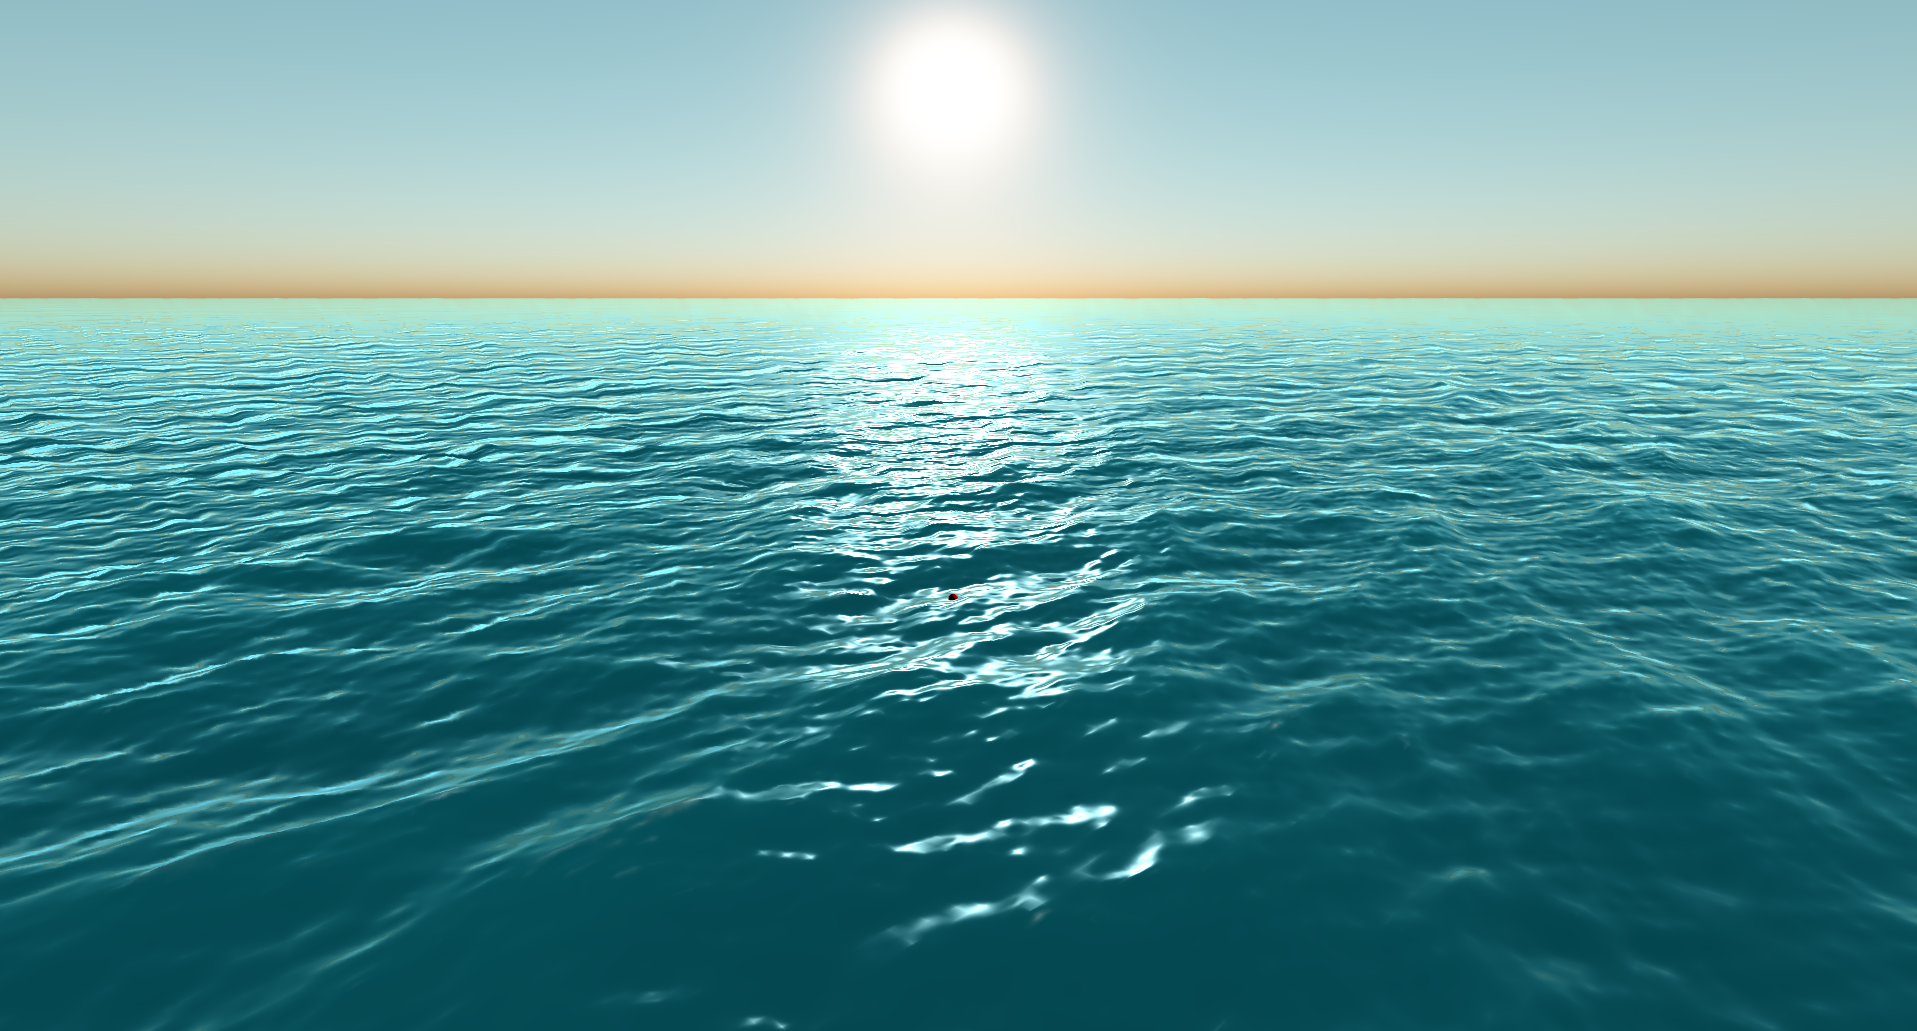
\includegraphics[width=0.8\textwidth]{img/ocean.png}
    \caption{Tensendorf waves in Nau3D Engine}
    \label{fig:tensendorf-waves-nau}
\end{figure}

% 2.
In this section we brief the Tensendorf waves demo in \autoref{subsec:tensendorf-waves} where we describe in which way FFTs are relevant for the implementation of this rendering technique, and how we improved an existing implementation for Nau3D that used a pass-per-stage Cooley-Tukey implementation. After that we present results and how the FFT implementation improves the demo performance and by how much in \autoref{subsec:results}.

\subsection{Tensendorf waves} \label{subsec:tensendorf-waves}

% FIXME: He calls it 'notes', what should I call it?  paper? article? other?
The rendering of the oceans demo we used as a starting point was a real-time implementation in Nau3D of the popular article published by \cite{tessendorf2001simulating}. In this demo there are two main stages, the generation of the height map and the actual rendering, the FFTs come into place in the generation of the height map since we need to generate it and the additional vectors used for shading. In total, there are $4$ 2D inverse FFTs computed for each frame, which translates to $8*FFT\_SIZE$ 1D FFTs in total.

% What previous strategies we apply and which ones we cant apply (such as the double real FFT, and double)

% Accordingly, the radix-2 and radix-4 Stockham algorithms were used, with the goal of studying the behavior of the multiple FFTs.
% \newline 


Regarding the results in \autoref{sec:glsl-implementation-results}, we first changed the pipeline from a pass-per-stage radix-2 Cooley-Tukey algorithm to implement radix-2 and radix-4 Stockham with synchronization within the kernel for the horizontal and vertical passes. Each pass computes multiple FFTs at a time and we take advantage of the same kernel to compute all required FFTs at the same time. Additionally, it is worth noticing that the inverse FFTs produce from the frequencies components, two usable real values. Finally, we used \texttt{vec4} as described in \autoref{sec:glsl-implementation-results} to compute multiple FFTs in the context of the SIMT instructions produced for the GPU. 
% NOTE: If needed, i can cite this > https://asawicki.info/news_1720_how_do_graphics_cards_execute_vector_instructions
%Within each \texttt{image2D} we store 2 complex values in a \texttt{vec4} so we also take advantage of SIMT operations optimize the additional cost. 

Although the FFTs take a big role in this demo, it also renders the ocean waves that have around 2 million vertices, hence, the performance does not only depend on the FFTs computation.
\newline


For this demo, we tested its performance with sizes $512$ and $1024$ for the ping pong buffers. We used size $512$ to test a balance of performance and wave quality and $1024$ to test for better wave quality as suggested by \cite{tessendorf2001simulating}.

Similarly to \autoref{sec:glsl-implementation-results}, the radix-4 Stockham implementation for the size $512$ integrates a final stage with radix-2 butterflies to be able to support the computation of this size.

%For this demo we used $512$ as the width for the 2D complex valued buffers, this width allows the waves to have good enough quality, however, \cite{tessendorf2001simulating} mentions we can increase the FFT size to $1024$ or $2048$ for better wave quality if needed. Accordingly, we also tested this demo with a width of $1024$ for more detailed waves and used radix-4 Stockham to achieve best performance.


\subsection{Results} \label{subsec:results}

\begin{figure}[H] 
    \begin{subfigure}{.5\textwidth}
        \centering
        \includegraphics[width=0.9\textwidth]{img/results/demo_cpu.png}
    \end{subfigure}
    \begin{subfigure}{.5\textwidth}
        \centering
        \includegraphics[width=0.9\textwidth]{img/results/demo_gpu.png}
    \end{subfigure}
    \caption{Time spent in the CPU and GPU for the size 512 FFT horizontal and vertical passes}
    \label{fig:demo}
\end{figure}

In \autoref{fig:demo} we can note the performance difference the radix-2 Stockham gives when performing the horizontal and vertical pass comparing it to the radix-2 Cooley-Tukey with a pass-per-stage. Not only is there an improvement in time and resources used by eliminating CPU steps, but there is also better performance using unique pass versions.

When running the application, the performance increase is noticeable and the frame rate is improved by up to 20\%.


% \begin{figure}[H] 
%     \begin{subfigure}{.5\textwidth}
%         \centering
%         \includegraphics[width=0.9\textwidth]{img/results/demo_1024_cpu.png}
%     \end{subfigure}
%     \begin{subfigure}{.5\textwidth}
%         \centering
%         \includegraphics[width=0.9\textwidth]{img/results/demo_1024_gpu.png}
%     \end{subfigure}
%     \caption{Total time spent in the CPU and GPU for the size 1024 FFT horizontal and vertical passes}
%     \label{fig:demo-1024}
% \end{figure}

Testing the demo for higher quality waves the radix-4 Stockham performance stands out in \autoref{fig:demo}, as predicted. When running the application, the difference in performance is noticeable, with the frame rate using Stockham radix-2 being improved by up to 20\%, while the radix-4 delivers a frame rate of up to 60\%.

These results proved the need to implement adequate algorithms to ensure the quality and performance of the target application.

These results proved the need to implement adequate algorithms to ensure the quality and performance of the application in question.

%%%%%%%%%%%%%%%%%%%%%%%%%%%%%%%%%%%%%%%%%%%%%%%%%%%%%%%%%%%%%%%%
%                 Conclusion and Future work                   %
%%%%%%%%%%%%%%%%%%%%%%%%%%%%%%%%%%%%%%%%%%%%%%%%%%%%%%%%%%%%%%%%
\chapter{Conclusions and Future work} \label{chap:conclusions-and-future-work}

In this thesis, we provided background on the Discrete Fourier Transform, with the goal of introducing the DIT and DIF Cooley-Tukey algorithms. From there, we described how the Stockham algorithm removes the need for the bit reversal permutation and what is the radix-4 of this algorithm. Moreover, we also discussed how a complex-valued FFT can be used to compute $2$ real-valued input sequences without any additional cost, and how this transformation can be applied to the spatial domain of a 2D image.

After presenting the Fast Fourier Transform and its algorithms, we processed implementing the Cooley-Tukey algorithm with a stage-per-pass approach followed by unique pass implementations of the radix-2 Cooley-Tukey and Stockham algorithm. Additionally, we also implemented the radix-4 Stockham algorithm, however, with the intent of having this algorithm support sizes of $2$ instead of just power of $4$, we altered the final stage of the code to conditionally implement a final stage of radix-2 Stockham.

Finally, to analyze these algorithms, we conducted a comparison of the performance of the implementations with benchmarks in a test environment and also measured implementation details such as the advantages and disadvantages of using stage-per-pass versus unique-pass and double the FFTs in GLSL by reusing the same \texttt{vec4} operations. From the compared algorithms, the best results were those of radix-4 Stockham, which we used as a model to test the possible benefits in the case study. The case study demonstrated positive results, by applying the previously discussed knowledge in the real-time rendering technique with radix-4 Stockham multiple FFTs.

\section{Results}

% UNIQUE-PASS APPROACH
% - Advantages:
%   - Synchronizes only on the GPU, and not with the CPU until the 2D FFT is fully calculated
%   - The work synchronizes only on the 1D FFT, and not on the whole 2D FFT, hence, it finishes the work earlier than the stage-per-pass approach
%   - Compute shader has more constant expressions and information, thus it is more prone to compiler optimizations
%   - If there is ...
% - Disadvantages:
%   - The implementation is specialized for some size
%   - Not as flexible to reuse this shader for other sizes
%   - Mixed radix cannot resize the invocation space 
%   - Higher kernel size
% BEST RESULTS RADIX-4 STOCKHAM
% - Stockham saves the bit reversal permutation
% - Memory access proves to be a problem, and radix-4 reduces the number of memory accesses by performing 2 radix-2 butterflies of 2 stages at once
% DOUBLE FFTS
% CASE STUDY
% - Produces 2 real, with double FFT using vec4

Based on the findings of \autoref{chap:analysis-and-comparison}, we were able to conclude several aspects of the tests carried out. When it comes to the tested unique-pass approach, it was demonstrated to be faster than the stage-per-pass, yet, we concluded multiple advantages and disadvantages:
\newline

Advantages:

\begin{itemize}
    \item Synchronization only on the GPU, and not with the CPU until the 2D FFT is fully calculated;
    \item The work synchronizes only on the 1D FFT, and not on the whole 2D FFT, hence, it finishes the work earlier than the stage-per-pass approach;
    \item Compute shader has more constant expressions and information, thus it is more prone to compiler optimizations.
\end{itemize}

Disadvantages:

\begin{itemize}
    \item Higher kernel size;
    \item The implementation is specialized for a specific size, therefore, not as flexible to reuse for other sizes. While the stage-per-pass implementation is reused for multiple power of $2$ sizes, the unique-pass strategies require changing the provided macro constants and recompiling as an additional shader;
    \item Mixed radix stages do not have special invocation spaces. This was the case of the radix-4 Stockham for power of $2$ sizes, we were required to use duplicate the amount of radix-2 Stockham stage performed by each thread since there were only $FFT\_SIZE/4$ threads.
\end{itemize}

Furthermore, when it comes to comparing implementations, it was found that radix-4 Stockham obtained the best results, up to $2 \times$ faster than radix-2 Cooley-Tukey. This was mainly due to the elimination of the bit reversal permutation and the reduction in the number of memory accesses by half due to the computation of $2$ radix-2 butterflies of $2$ radix-2 stages at once.

When the acquired knowledge was applied to the case study, as expected, there was an increase in performance similar to that of the tests carried out. This case study applied strategies that were described and tested, such as the use of double FFTs by using the \texttt{vec4} operations and the multiple real values from the FFT frequencies. The results improved the frames per second of the application by up to 60\%.

\section{Future work}

% - IMPROVE MEMORY ACCESS
% - EXPERIMENT WITH HIGHER RADIX 
%   - For multiple GPUs
%   - On average, for each size what combinations of radix suits best?
%   - With unique-pass, stage-per-pass and mixed approaches

With the obtained results, other questions arise, which may lead to future studies to expand the work carried out.

Although the radix-4 reduced the memory accesses by half, these memory loads still weigh on the performance of the compute shaders, other strategies for this problem could be studied to reduce the overhead this introduces.

Since the results of the radix-4 Stockham were the fastest when using radix higher than 4, what is the most suitable configuration for dispatching a higher radix implementation while still supporting power of $2$ sizes? With the size restriction of the invocation space until the kernel is done executing, the unique-pass approach needs to duplicate the number of butterflies for each lower radix stage of the implementation. Therefore, we could study the implementation of these higher radix algorithms to verify if the usage of stage passes for the lower radix stages would be more beneficial than strictly having a unique-pass approach. A study could be carried out to explore these conditions for multiple GPUs, and come to a conclusion on the best configuration on average for the tested hardware.


%%%%%%%%%%%%%%%%%%%%%%%%%%%%%%%%%%%%%%%%%%%%%%%%%%%%%%%%%%%%%%%%
%                     END OF MAIN CHAPTERS                     %
%%%%%%%%%%%%%%%%%%%%%%%%%%%%%%%%%%%%%%%%%%%%%%%%%%%%%%%%%%%%%%%%

\bookmarksetup{startatroot} % Ends last part.
% \addtocontents{toc}{\bigskip} % Making the table of contents look good.
\cleardoublepage

% Bibliography (requires 'bibtex'  package)
\addcontentsline{toc}{chapter}{Bibliography}
\bibliographystyle{acm}
\bibliography{dissertation}
% Index of terms (required 'makeindex' package)
\printindex

    \appendix
    \renewcommand\chaptername{Appendix}

    % Add appendix chapters

%%%%%%%%%%%%%%%%%%%%%%%%%%%%%%%%%%%%%%%%%%%%%%%%%%%%%%%%%%%%%%%%%

\part{Appendices}

\chapter{GLSL FFT} \label{apdx:glsl-fft}

\begin{lstlisting}[language=C,caption={FFT Radix-2 Cooley-Tukey Horizontal stage pass, see \autoref{sec:ct-impl}},label={lst:glsl-radix2-ct-stage-horizontal}]
 #version 440
 
 #define M_PI 3.1415926535897932384626433832795
 
 layout (local_size_x = 4, local_size_y = 8) in;
 
 layout (binding = 0, rg32f) uniform image2D pingpong0;
 layout (binding = 0, rg32f) uniform image2D pingpong1;
 
 uniform int pingpong;
 uniform int log_width;
 uniform int stage;
 uniform int fft_dir;
 
 vec2 complex_mult(vec2 v0, vec2 v1) {
 	return vec2(v0.x * v1.x - v0.y * v1.y,
 				v0.x * v1.y + v0.y * v1.x);
 }
 
 int bit_reverse(int k) {
     uint br = bitfieldReverse(k);
     return int(bitfieldExtract(br, 32 - log_width, log_width));
 }
 
 vec2 euler(float angle) {
 	return vec2(cos(angle), sin(angle));
 }
 
 void main() {
 	int line = int(gl_GlobalInvocationID.x);
 	int column = int(gl_GlobalInvocationID.y);
 
 	int group_size = 2 << stage;
 	int shift = 1 << stage;
 
 	vec2 a, b;
 
     int idx = (line % shift) + group_size * (line / shift);
     vec2 w = euler(fft_dir * 2 * (M_PI / group_size) * ((idx % group_size) % shift));
 
     if (pingpong == 0) {
         if (stage == 0) {
             a = imageLoad(pingpong0, ivec2(bit_reverse(idx), column)).rg;
             b = imageLoad(pingpong0, ivec2(bit_reverse(idx + shift), column)).rg;
         }
         else {
             a = imageLoad(pingpong0, ivec2(idx, column)).rg;
             b = imageLoad(pingpong0, ivec2(idx + shift, column)).rg;
         }

         vec2 wb = complex_mult(w, b);
         vec2 raux = a + wb;
         imageStore(pingpong1, ivec2(idx, column), vec4(raux, 0, 0));
             
         raux = a - wb;
         imageStore(pingpong1, ivec2(idx + shift, column), vec4(raux, 0, 0));
     }
     else {
         a = imageLoad(pingpong1, ivec2(idx, column)).rg;
         b = imageLoad(pingpong1, ivec2(idx + shift, column)).rg;

         vec2 wb = complex_mult(w, b);
         vec2 raux = a + wb;
         imageStore(pingpong0, ivec2(idx, column), vec4(raux,0,0));
             
         raux = a - wb;
         imageStore(pingpong0, ivec2(idx + shift, column), vec4(raux,0,0));
     }
 }
\end{lstlisting}

% TODO: Maybe remove the error checks for a less verbose listing

\begin{lstlisting}[language=C,caption={FFT Radix-2 Cooley-Tukey Vertical stage pass, see \autoref{sec:ct-impl}},label={lst:glsl-radix2-ct-stage-vertical}]
#version 440

#define M_PI 3.1415926535897932384626433832795

layout (local_size_x = 8, local_size_y = 4) in;

layout (binding = 0, rg32f) uniform image2D pingpong0;
layout (binding = 1, rg32f) uniform image2D pingpong1;

uniform int pingpong;
uniform int log_width;
uniform int stage;
uniform int fft_dir;

int iter = 1 << log_width;
int shift = (1 << stage);

vec2 complex_mult(vec2 v0, vec2 v1) {
	return vec2(v0.x * v1.x - v0.y * v1.y,
				v0.x * v1.y + v0.y * v1.x);
}

int bit_reverse(int k) {
    uint br = bitfieldReverse(k);
    return int(bitfieldExtract(br, 32 - log_width, log_width));
}

vec2 euler(float angle) {
	return vec2(cos(angle), sin(angle));
}

void main() {
	int line = int(gl_GlobalInvocationID.x);
	int column = int(gl_GlobalInvocationID.y);

	int group_size = 2 << stage;
	int shift = 1 << stage;

	vec2 a, b;

    int idx = (column % shift) + group_size * (column / shift);
    vec2 w = euler(fft_dir * 2 * (M_PI / group_size) * ((idx % group_size) % shift));

    float mult_factor = 1.0;
    if ((stage == log_width - 1) && fft_dir == 1) {
        mult_factor = 1.0 / (iter*iter) ;
    }

    if (pingpong == 0) {
        if (stage == 0) {
            a = imageLoad(pingpong0, ivec2(line, bit_reverse(idx))).rg;
            b = imageLoad(pingpong0, ivec2(line, bit_reverse(idx + shift))).rg;
        }
        else {
            a = imageLoad(pingpong0, ivec2(line, idx)).rg;
            b = imageLoad(pingpong0, ivec2(line, idx + shift)).rg;
        }

        vec2 wb = complex_mult(w, b);
        vec2 raux = (a + wb) * mult_factor;
        imageStore(pingpong1, ivec2(line, idx), vec4(raux,0,0));
            
        raux = (a - wb) * mult_factor;
        imageStore(pingpong1, ivec2(line, idx + shift), vec4(raux,0,0));
    }
    else {
        if (stage == 0) {
            a = imageLoad(pingpong1, ivec2(line, bit_reverse(idx))).rg;
            b = imageLoad(pingpong1, ivec2(line, bit_reverse(idx + shift))).rg;
        }
        else {	
            a = imageLoad(pingpong1, ivec2(line, idx)).rg;
            b = imageLoad(pingpong1, ivec2(line, idx + shift)).rg;
        }

        vec2 wb = complex_mult(w, b);
        vec2 raux = (a + wb) * mult_factor;
        imageStore(pingpong0, ivec2(line, idx), vec4(raux,0,0));
            
        raux = (a - wb) * mult_factor;
        imageStore(pingpong0, ivec2(line, idx + shift), vec4(raux,0,0));
    }
}
\end{lstlisting}

\begin{lstlisting}[language=C,caption={FFT Radix-2 Cooley-Tukey Horizontal unique pass, see \autoref{subsec:all-stages-in-one-pass}},label={lst:glsl-radix2-ct-unique-horizontal}]
#version 440

#define M_PI 3.1415926535897932384626433832795
#define FFT_SIZE 256
#define LOG_SIZE 8

layout (local_size_x = FFT_SIZE/2, local_size_y = 1) in;

layout (binding = 0, rg32f) uniform image2D pingpong0;
layout (binding = 1, rg32f) uniform image2D pingpong1;

uniform int fft_dir;

vec2 complex_mult(vec2 v0, vec2 v1) {
    return vec2(v0.x * v1.x - v0.y * v1.y,
                v0.x * v1.y + v0.y * v1.x);
}

int bit_reverse(int k) {
    uint br = bitfieldReverse(k);
    return int(bitfieldExtract(br, 32 - LOG_SIZE, LOG_SIZE));
}

vec2 euler(float angle) {
    return vec2(cos(angle), sin(angle));
}

void main() {
    int line = int(gl_GlobalInvocationID.x);
    int column = int(gl_WorkGroupID.y);
    int pingpong = 0;
    
    for(int stage = 0; stage < LOG_SIZE; ++stage) {
        int group_size = 2 << stage;
        int shift = 1 << stage;

        vec2 a, b;
        int idx = (line % shift) + group_size * (line / shift);
        vec2 w = euler(fft_dir * 2 * (M_PI / group_size) * ((idx % group_size) % shift));

        // alternate between textures
        if (pingpong == 0) {
            if (stage == 0) {
                a = imageLoad(pingpong0, ivec2(bit_reverse(idx), column)).rg;
                b = imageLoad(pingpong0, ivec2(bit_reverse(idx + shift), column)).rg;
            }
            else {
                a = imageLoad(pingpong0, ivec2(idx, column)).rg;
                b = imageLoad(pingpong0, ivec2(idx + shift, column)).rg;
            }

            vec2 wb = complex_mult(w, b);
            vec2 raux = a + wb;
            imageStore(pingpong1, ivec2(idx, column), vec4(raux, 0, 0));
            raux = a - wb;
            imageStore(pingpong1, ivec2(idx + shift, column), vec4(raux, 0, 0));
        }
        else {
            a = imageLoad(pingpong1, ivec2(idx, column)).rg;
            b = imageLoad(pingpong1, ivec2(idx + shift, column)).rg;

            vec2 wb = complex_mult(w, b);
            vec2 raux = a + wb;
            imageStore(pingpong0, ivec2(idx, column), vec4(raux,0,0));
            raux = a - wb;
            imageStore(pingpong0, ivec2(idx + shift, column), vec4(raux,0,0));
        }

        pingpong = (pingpong + 1) % 2;
        barrier();
    }
}
\end{lstlisting}

\begin{lstlisting}[language=C,caption={FFT Radix-2 Cooley-Tukey Vertical unique pass, see \autoref{subsec:all-stages-in-one-pass}},label={lst:glsl-radix2-ct-unique-vertical}]
#version 440

#define M_PI 3.1415926535897932384626433832795
#define FFT_SIZE 256
#define LOG_SIZE 8

layout (local_size_x = FFT_SIZE/2, local_size_y = 1) in;

layout (binding = 0, rg32f) uniform image2D pingpong0;
layout (binding = 1, rg32f) uniform image2D pingpong1;

uniform int fft_dir;

vec2 complex_mult(vec2 v0, vec2 v1) {
	return vec2(v0.x * v1.x - v0.y * v1.y,
				v0.x * v1.y + v0.y * v1.x);
}

int bit_reverse(int k) {
    uint br = bitfieldReverse(k);
    return int(bitfieldExtract(br, 32 - LOG_SIZE, LOG_SIZE));
}

vec2 euler(float angle) {
	return vec2(cos(angle), sin(angle));
}

void main() {
	int line = int(gl_WorkGroupID.y);
	int column = int(gl_GlobalInvocationID.x);
    int pingpong = LOG_SIZE % 2;

    for(int stage = 0; stage < LOG_SIZE; ++stage) {
        int group_size = 2 << stage;
        int shift = 1 << stage;
        
        vec2 a, b;
        int idx = (column % shift) + group_size * (column / shift);
        vec2 w = euler(fft_dir * 2 * (M_PI / group_size) * ((idx % group_size) % shift));

        float mult_factor = 1.0;
        if ((stage == LOG_SIZE - 1) && fft_dir == 1) {
            mult_factor = 1.0 / (FFT_SIZE*FFT_SIZE);
        }

        if (pingpong == 0) {
            if (stage == 0) {
                a = imageLoad(pingpong0, ivec2(line, bit_reverse(idx))).rg;
                b = imageLoad(pingpong0, ivec2(line, bit_reverse(idx + shift))).rg;
            }
            else {
                a = imageLoad(pingpong0, ivec2(line, idx)).rg;
                b = imageLoad(pingpong0, ivec2(line, idx + shift)).rg;
            }

            vec2 wb = complex_mult(w, b);
            vec2 raux = (a + wb) * mult_factor;
            imageStore(pingpong1, ivec2(line, idx), vec4(raux,0,0));
            raux = (a - wb) * mult_factor;
            imageStore(pingpong1, ivec2(line, idx + shift), vec4(raux,0,0));

        }
        else {
            if (stage == 0) {
                a = imageLoad(pingpong1, ivec2(line, bit_reverse(idx))).rg;
                b = imageLoad(pingpong1, ivec2(line, bit_reverse(idx + shift))).rg;
            }
            else {	
                a = imageLoad(pingpong1, ivec2(line, idx)).rg;
                b = imageLoad(pingpong1, ivec2(line, idx + shift)).rg;
            }

            vec2 wb = complex_mult(w, b);
            vec2 raux = (a + wb) * mult_factor;
            imageStore(pingpong0, ivec2(line, idx), vec4(raux,0,0));
            raux = (a - wb) * mult_factor;
            imageStore(pingpong0, ivec2(line, idx + shift), vec4(raux,0,0));
        }
        
        pingpong = ((pingpong + 1) % 2);
        barrier();
    }
}
\end{lstlisting}

\begin{lstlisting}[language=C, caption={FFT Radix-2 Stockham Horizontal unique pass, see \autoref{sec:radix2-stockham}}, label={lst:glsl-radix2-stockham-horizontal}]
#version 440

#define M_PI 3.1415926535897932384626433832795
#define FFT_SIZE 256
#define LOG_SIZE 8

layout (local_size_x = (FFT_SIZE/2)/NUM_BUTTERFLIES, local_size_y = 1) in;

layout (binding = 0, rg32f) uniform image2D pingpong0;
layout (binding = 1, rg32f) uniform image2D pingpong1;

uniform int fft_dir;

vec2 complex_mult(vec2 v0, vec2 v1) {
    return vec2(v0.x * v1.x - v0.y * v1.y,
                v0.x * v1.y + v0.y * v1.x);
}

vec2 euler(float angle) {
    return vec2(cos(angle), sin(angle));
}

void main() {
    int line = int(gl_GlobalInvocationID.x);
    int column = int(gl_WorkGroupID.y);
    int pingpong = 0;

    for(int stage = 0; stage < LOG_SIZE; ++stage) {
        int n = 1 << (LOG_SIZE - stage);
        int m = n >> 1;
        int s = 1 << stage;

        int p = line / s;
        int q = line % s;
            
        vec2 wp = euler(fft_dir * 2 * (M_PI / n) * p);
        if(pingpong == 0) {
            vec2 a = imageLoad(pingpong0, ivec2(q + s*(p + 0), column)).rg;
            vec2 b = imageLoad(pingpong0, ivec2(q + s*(p + m), column)).rg;

            vec2 res = (a + b);
            imageStore(pingpong1, ivec2(q + s*(2*p + 0), column), vec4(res,0,0));
            res = complex_mult(wp,(a - b));
            imageStore(pingpong1, ivec2(q + s*(2*p + 1), column), vec4(res,0,0));
        }
        else {
            vec2 a = imageLoad(pingpong1, ivec2(q + s*(p + 0), column)).rg;
            vec2 b = imageLoad(pingpong1, ivec2(q + s*(p + m), column)).rg;

            vec2 res = (a + b);
            imageStore(pingpong0, ivec2(q + s*(2*p + 0), column), vec4(res,0,0));
            res = complex_mult(wp,(a - b));
            imageStore(pingpong0, ivec2(q + s*(2*p + 1), column), vec4(res,0,0));
        }
        
        pingpong = (pingpong + 1) % 2;
        barrier();
    }
}
\end{lstlisting}

\begin{lstlisting}[language=C, caption={FFT Radix-2 Stockham Vertical unique pass, see \autoref{sec:radix2-stockham}}, label={lst:glsl-radix2-stockham-vertical}]
#version 440

#define M_PI 3.1415926535897932384626433832795
#define FFT_SIZE 256
#define LOG_SIZE 8

layout (local_size_x = FFT_SIZE/2, local_size_y = 1) in;

layout (binding = 0, rg32f) uniform image2D pingpong0;
layout (binding = 1, rg32f) uniform image2D pingpong1;

uniform int fft_dir;

vec2 complex_mult(vec2 v0, vec2 v1) {
	return vec2(v0.x * v1.x - v0.y * v1.y,
				v0.x * v1.y + v0.y * v1.x);
}

vec2 euler(float angle) {
	return vec2(cos(angle), sin(angle));
}

void main() {
	int line = int(gl_WorkGroupID.y);
	int column = int(gl_GlobalInvocationID.x);
    int pingpong = LOG_SIZE % 2;

    for(int stage = 0; stage < LOG_SIZE; ++stage) {
        int n = 1 << (LOG_SIZE - stage);
        int m = n >> 1;
        int s = 1 << stage;

	    float mult_factor = 1.0;
	    if ((stage == LOG_SIZE-1) && fft_dir == 1) {
	    	mult_factor = 1.0 / (FFT_SIZE*FFT_SIZE) ;
	    }

        int p = column / s;
        int q = column % s;

        vec2 wp = euler(fft_dir * 2 * (M_PI / n) * p);
        if(pingpong == 0) {
            vec2 a = imageLoad(pingpong0, ivec2(line, q + s*(p + 0))).rg;
            vec2 b = imageLoad(pingpong0, ivec2(line, q + s*(p + m))).rg;

            vec2 res = (a + b) * mult_factor;
            imageStore(pingpong1, ivec2(line, q + s*(2*p + 0)), vec4(res,0,0));
            res = complex_mult(wp,(a - b)) * mult_factor;
            imageStore(pingpong1, ivec2(line, q + s*(2*p + 1)), vec4(res,0,0));
        }
        else {
            vec2 a = imageLoad(pingpong1, ivec2(line, q + s*(p + 0))).rg;
            vec2 b = imageLoad(pingpong1, ivec2(line, q + s*(p + m))).rg;

            vec2 res = (a + b) * mult_factor;
            imageStore(pingpong0, ivec2(line, q + s*(2*p + 0)), vec4(res,0,0));
            res = complex_mult(wp,(a - b)) * mult_factor;
            imageStore(pingpong0, ivec2(line, q + s*(2*p + 1)), vec4(res,0,0));
        }

        pingpong = (pingpong + 1) % 2;
        barrier();
    }
}
\end{lstlisting}

\begin{lstlisting}[language=C, caption={FFT Radix-4 Stockham Horizontal unique pass, see \autoref{subsec:radix4-stockham}}, label={lst:glsl-radix4-stockham-horizontal}]
#version 440

#define M_PI 3.1415926535897932384626433832795
#define FFT_SIZE 256
#define LOG_SIZE 8 // log2(FFT_SIZE)
#define HALF_LOG_SIZE 4 // log2(FFT_SIZE) / 2

layout (local_size_x = FFT_SIZE/4, local_size_y = 1) in;

layout (binding = 0, rg32f) uniform image2D pingpong0;
layout (binding = 1, rg32f) uniform image2D pingpong1;

uniform int fft_dir;

vec2 complex_mult(vec2 v0, vec2 v1) {
    return vec2(v0.x * v1.x - v0.y * v1.y,
                v0.x * v1.y + v0.y * v1.x);
}

vec2 euler(float angle) {
    return vec2(cos(angle), sin(angle));
}

void main() {
    int line = int(gl_GlobalInvocationID.x);
    int column = int(gl_WorkGroupID.y);
    int pingpong = 0;

    for(int stage = 0; stage < HALF_LOG_SIZE; ++stage) {
        int n = 1 << (HALF_LOG_SIZE - stage)*2;
        int s = 1 << stage*2;

        int n0 = 0;
        int n1 = n/4;
        int n2 = n/2;
        int n3 = n1 + n2;

        int p = line / s;
        int q = line % s;

        vec2 w1p = euler(2*(M_PI / n) * p * fft_dir);
        vec2 w2p = complex_mult(w1p,w1p);
        vec2 w3p = complex_mult(w1p,w2p);

        if(pingpong == 0) {
            vec2 a = imageLoad(pingpong0, ivec2(q + s*(p + n0), column)).rg;
            vec2 b = imageLoad(pingpong0, ivec2(q + s*(p + n1), column)).rg;
            vec2 c = imageLoad(pingpong0, ivec2(q + s*(p + n2), column)).rg;
            vec2 d = imageLoad(pingpong0, ivec2(q + s*(p + n3), column)).rg;

            vec2 apc = a + c;
            vec2 amc = a - c;
            vec2 bpd = b + d;
            vec2 jbmd = complex_mult(vec2(0,1), b - d);

            imageStore(pingpong1, ivec2(q + s*(4*p + 0), column), vec4(apc + bpd, 0,0));
            imageStore(pingpong1, ivec2(q + s*(4*p + 1), column), vec4(complex_mult(w1p, amc + jbmd*fft_dir), 0,0));
            imageStore(pingpong1, ivec2(q + s*(4*p + 2), column), vec4(complex_mult(w2p, apc - bpd ), 0,0));
            imageStore(pingpong1, ivec2(q + s*(4*p + 3), column), vec4(complex_mult(w3p, amc - jbmd*fft_dir), 0,0));
        }
        else {
            vec2 a = imageLoad(pingpong1, ivec2(q + s*(p + n0), column)).rg;
            vec2 b = imageLoad(pingpong1, ivec2(q + s*(p + n1), column)).rg;
            vec2 c = imageLoad(pingpong1, ivec2(q + s*(p + n2), column)).rg;
            vec2 d = imageLoad(pingpong1, ivec2(q + s*(p + n3), column)).rg;

            vec2 apc = a + c;
            vec2 amc = a - c;
            vec2 bpd = b + d;
            vec2 jbmd = complex_mult(vec2(0,1), b - d);

            imageStore(pingpong0, ivec2(q + s*(4*p + 0), column), vec4(apc + bpd, 0,0));
            imageStore(pingpong0, ivec2(q + s*(4*p + 1), column), vec4(complex_mult(w1p, amc + jbmd*fft_dir), 0,0));
            imageStore(pingpong0, ivec2(q + s*(4*p + 2), column), vec4(complex_mult(w2p, apc - bpd ), 0,0));
            imageStore(pingpong0, ivec2(q + s*(4*p + 3), column), vec4(complex_mult(w3p, amc - jbmd*fft_dir), 0,0));
        }
        

        pingpong = (pingpong + 1) % 2;
        barrier();
    }
}
\end{lstlisting}

\begin{lstlisting}[language=C, caption={FFT Radix-4 Stockham Vertical unique pass, see \autoref{subsec:radix4-stockham}}, label={lst:glsl-radix4-stockham-vertical}]
#version 440

#define M_PI 3.1415926535897932384626433832795
#define FFT_SIZE 256
#define LOG_SIZE 8 // log2(FFT_SIZE)
#define HALF_LOG_SIZE 4 // log2(FFT_SIZE) / 2

layout (local_size_x = (FFT_SIZE/4)/NUM_BUTTERFLIES, local_size_y = 1) in;

layout (binding = 0, rg32f) uniform image2D pingpong0;
layout (binding = 1, rg32f) uniform image2D pingpong1;

uniform int fft_dir;

vec2 complex_mult(vec2 v0, vec2 v1) {
	return vec2(v0.x * v1.x - v0.y * v1.y,
				v0.x * v1.y + v0.y * v1.x);
}

vec2 euler(float angle) {
	return vec2(cos(angle), sin(angle));
}

void main() {
	int line = int(gl_WorkGroupID.y);
	int column = int(gl_GlobalInvocationID.x);
    int pingpong = HALF_LOG_SIZE % 2;

    for(int stage = 0; stage < HALF_LOG_SIZE; ++stage) {
        int group_size = 2 << stage;
        int shift = 1 << stage;

        int n = 1 << ((HALF_LOG_SIZE - stage)*2);
        int s = 1 << (stage*2);

        int n0 = 0;
        int n1 = n/4;
        int n2 = n/2;
        int n3 = n1 + n2;

	    float mult_factor = 1.0;
	    if((stage == HALF_LOG_SIZE - 1) && fft_dir == 1) {
	    	mult_factor = 1.0 / (FFT_SIZE*FFT_SIZE) ;
	    }

        int p = column / s;
        int q = column % s;

        vec2 w1p = euler(2*(M_PI / n) * p * fft_dir);
        vec2 w2p = complex_mult(w1p,w1p);
        vec2 w3p = complex_mult(w1p,w2p);

        if(pingpong == 0) {
            vec2 a = imageLoad(pingpong0, ivec2(line, q + s*(p + n0))).rg;
            vec2 b = imageLoad(pingpong0, ivec2(line, q + s*(p + n1))).rg;
            vec2 c = imageLoad(pingpong0, ivec2(line, q + s*(p + n2))).rg;
            vec2 d = imageLoad(pingpong0, ivec2(line, q + s*(p + n3))).rg;

            vec2 apc = a + c;
            vec2 amc = a - c;
            vec2 bpd = b + d;
            vec2 jbmd = complex_mult(vec2(0,1), b - d);

            imageStore(pingpong1, ivec2(line, q + s*(4*p + 0)), vec4(mult_factor * (apc + bpd), 0,0));
            imageStore(pingpong1, ivec2(line, q + s*(4*p + 1)), vec4(mult_factor * (complex_mult(w1p, amc + jbmd*fft_dir)), 0,0));
            imageStore(pingpong1, ivec2(line, q + s*(4*p + 2)), vec4(mult_factor * (complex_mult(w2p, apc - bpd )), 0,0));
            imageStore(pingpong1, ivec2(line, q + s*(4*p + 3)), vec4(mult_factor * (complex_mult(w3p, amc - jbmd*fft_dir)), 0,0));
        }
        else {
            vec2 a = imageLoad(pingpong1, ivec2(line, q + s*(p + n0))).rg;
            vec2 b = imageLoad(pingpong1, ivec2(line, q + s*(p + n1))).rg;
            vec2 c = imageLoad(pingpong1, ivec2(line, q + s*(p + n2))).rg;
            vec2 d = imageLoad(pingpong1, ivec2(line, q + s*(p + n3))).rg;

            vec2 apc = a + c;
            vec2 amc = a - c;
            vec2 bpd = b + d;
            vec2 jbmd = complex_mult(vec2(0,1), b - d);

            imageStore(pingpong0, ivec2(line, q + s*(4*p + 0)), vec4(mult_factor * (apc + bpd), 0,0));
            imageStore(pingpong0, ivec2(line, q + s*(4*p + 1)), vec4(mult_factor * (complex_mult(w1p, amc + jbmd*fft_dir)), 0,0));
            imageStore(pingpong0, ivec2(line, q + s*(4*p + 2)), vec4(mult_factor * (complex_mult(w2p, apc - bpd )), 0,0));
            imageStore(pingpong0, ivec2(line, q + s*(4*p + 3)), vec4(mult_factor * (complex_mult(w3p, amc - jbmd*fft_dir)), 0,0));
        }

        pingpong = (pingpong + 1) % 2;
        barrier();
    }
}
\end{lstlisting}

\chapter{cuFFT} \label{apdx:cufft}

\begin{lstlisting}[language=C++,caption={cuFFT, see \autoref{sec:cufft}},label={lst:cufft}]
#include <cstdio>
#include <cufft.h>
#include <cuda.h>

#define FFT_SIZE 256

#define CU_ERR_CHECK_MSG(err, msg) {       \
    if(err != cudaSuccess) {               \
        fprintf(stderr, msg);              \
        exit(1);                           \
    }                                      \
}

#define CU_CHECK_MSG(res, msg) {           \
    if(res != CUFFT_SUCCESS) {             \
        fprintf(stderr, msg);              \
        exit(1);                           \
    }                                      \
}

int main() {
    const size_t data_size = sizeof(cufftComplex)*FFT_SIZE*FFT_SIZE;
    cufftComplex* data = reinterpret_cast<cufftComplex*>(malloc(data_size));
    cufftComplex* gpu_data_in;
    cufftComplex* gpu_data_out;
    cudaError_t err;
    
    // Initializing input sequence
    for(size_t i = 0; i < FFT_SIZE*FFT_SIZE; ++i) {
        data[i].x = i;
        data[i].y = 0.00;
    }
    
    // Allocate Input GPU buffer
    err = cudaMalloc(&gpu_data_in, data_size);
    CU_ERR_CHECK_MSG(err, "Cuda error: Failed to allocate\n");
    
    // Allocate Output GPU buffer
    err = cudaMalloc(&gpu_data_out, data_size);
    CU_ERR_CHECK_MSG(err, "Cuda error: Failed to allocate\n");
    
    // Copy data to GPU buffer
    err = cudaMemcpy(gpu_data_in, data, data_size, cudaMemcpyHostToDevice);
    CU_ERR_CHECK_MSG(err, "Cuda error: Failed to copy buffer to GPU\n");
    
    // Setup cufft plan
    cufftHandle plan;
    cufftResult_t res;
    res = cufftPlan2d(&plan, FFT_SIZE, FFT_SIZE, CUFFT_C2C);
    CU_CHECK_MSG(res, "cuFFT error: Plan creation failed\n");
    
    // Execute Forward 2D FFT
    res = cufftExecC2C(plan, gpu_data_in, gpu_data_out, CUFFT_FORWARD);
    CU_CHECK_MSG(res, "cuFFT error: ExecC2C Forward failed\n");
    
    // Await end of execution
    err = cudaDeviceSynchronize();
    CU_ERR_CHECK_MSG(err, "Cuda error: Failed to synchronize\n");
    
    // Execute Inverse 2D FFT
    res = cufftExecC2C(plan, gpu_data_in, gpu_data_out, CUFFT_FORWARD);
    CU_CHECK_MSG(res, "cuFFT error: ExecC2C Forward failed\n");
    
    // Await end of execution
    err = cudaDeviceSynchronize();
    CU_ERR_CHECK_MSG(err, "Cuda error: Failed to synchronize\n");
    
    // Retrieve computed FFT buffer
    err = cudaMemcpy(data, gpu_data_in, data_size, cudaMemcpyDeviceToHost);
    CU_ERR_CHECK_MSG(err, "Cuda error: Failed to copy buffer to GPU\n");
    
    // Destroy Cuda and cuFFT resources
    cufftDestroy(plan);
    cudaFree(gpu_data_in);

    return 0;
}
\end{lstlisting}

%%%%%%%%%%%%%%%%%%%%%%%%%%%%%%%%%%%%%%%%%%%%%%%%%%%%%%%%%%%%%%%%%

% \chapter{Support work}
% 	Auxiliary results which are not main-stream

%%%%%%%%%%%%%%%%%%%%%%%%%%%%%%%%%%%%%%%%%%%%%%%%%%%%%%%%%%%%%%%%%

% \chapter{Details of results}
%          Details of results whose length would compromise readability of main text.

%%%%%%%%%%%%%%%%%%%%%%%%%%%%%%%%%%%%%%%%%%%%%%%%%%%%%%%%%%%%%%%%%

% \chapter{Listings}
% 	Should this be the case

%%%%%%%%%%%%%%%%%%%%%%%%%%%%%%%%%%%%%%%%%%%%%%%%%%%%%%%%%%%%%%%%%

% \chapter{Tooling}
% 	(Should this be the case)

% 	Anyone using \Latex\ should consider having a look at \TUG,
% 	the \tug{\TeX\ Users Group}

%%%%%%%%%%%%%%%%%%%%%%%%%%%%%%%%%%%%%%%%%%%%%%%%%%%%%%%%%%%%%%%%%

% \begin{backcover}
% \thispagestyle{empty} \pagecolor{white} \textcolor{black} {\fontfamily{phv}\fontseries{mc}\selectfont ~\vfill
% \noindent
% NB: place here information about funding, FCT project, etc in which the work is framed. Leave empty otherwise.
% %
% \vfill ~}
% \end{backcover}

\end{document}
